\documentclass[11pt]{article}

\usepackage[tt=false, type1=true]{libertine}
\usepackage[varqu]{zi4}
\usepackage[libertine]{newtxmath}
\usepackage[T1]{fontenc}

\let\openbox\relax
\usepackage{amsthm}
\usepackage[pdftex]{graphicx}
\usepackage{url}
\usepackage{color,xcolor,colortbl}
\usepackage{algorithm}
\usepackage[mathscr]{euscript}		% DO NOT remove this line, otherwise some symbols may get overload!
\usepackage[letterpaper]{geometry}
\geometry{verbose,tmargin=1in,bmargin=1in,lmargin=1in,rmargin=1in}

\definecolor{darkblue}{rgb}{0.0,0.0,0.5}
\usepackage[unicode=true,bookmarks=true,bookmarksnumbered=false,bookmarksopen=true,hidelinks=true,colorlinks=true,citecolor=darkblue,linkcolor=black]{hyperref}
	
\usepackage{epstopdf}
\usepackage{relsize}
\usepackage{slashbox}
\usepackage{algpseudocode}

\newcommand{\etal}{\textit{et~al.}}
\newcommand{\eg}{\textit{e.g.}}
\newcommand{\ie}{\textit{i.e.}}
\newcommand{\alg}[1]{\mbox{\textsf{#1}}}
\newcommand{\view}[1]{\textsf{{\small VIEW}}_{#1}}

\setlength{\parskip}{0.25em}
\let \labelindent \relax
\usepackage{enumitem}
\setlist[description]{listparindent=\parindent,leftmargin=0em,itemsep=1em}

\newtheorem{theorem}{Theorem}
\newtheorem{lemma}{Lemma}
\newtheorem{corollary}{Corollary}
\newtheorem{definition}{Definition}
\floatname{algorithm}{Protocol}
\theoremstyle{plain}

% angled brackets
\newcommand{\ang}[1]{\langle #1 \rangle}

% disables hyperlinks
\newcommand{\nohyperlinks}{\hypersetup{hidelinks}}

% use Sans-Serif font throughout the document
\newcommand{\sansfont}{\renewcommand{\familydefault}{\sfdefault}}

\newcommand{\softO}[1]{\tilde O(#1)}				% soft-O
\newcommand{\poly}[1]{\mathsf{poly}(#1)}			% poly
\newcommand{\polylog}[1]{\mathsf{polylog}(#1)}		% polylog

% author comments
\newcommand{\xcomment}[2]{[{\textcolor{blue}{\underline{\bf #1:}}} {\bf \em #2}]}
\newcommand{\mahdi}[1]{\xcomment{Mahdi}{#1}}

\begin{document}

\title{Notes on Cryptography and Computer Security}

\author{Mahdi Zamani\\ Visa Research, Palo Alto, CA \\ \textit{mzamani@visa.com}}
\date{}

\maketitle

\section{Introduction}

In provable security, we prove that no adversary exists that can break
the security of a scheme. To do this, we first need to define \emph{notions
	of security} that clearly define adversary's goals and how much power
and information it is given. We also need to choose our \emph{proof
	models}, which clearly define the set of assumptions that help us
proof the security of our algorithms. One also needs to define a \emph{communication
	model}, which describes how the communication channels used by participants
in a protocol behave. In this section, we describe various such models
that are used frequently in cryptography and distributed algorithms
communities.

\subsection{Notions of Security}

In terms of its computational power, an adversary can be categorized
as one of the following types:
\begin{itemize}
	\item \textbf{Computationally-bounded.} An adversary who is capable of only
	polynomial-time computation. A model with this type of adversary provides
	computational security.
	\item \textbf{Computationally-unbounded.} An adversary who has \emph{unknown}
	(not necessarily infinite) amounts of resources. Thus, any algorithm
	in this model cannot assume any bound on the adversary's computational
	powers and it must maintain its security with \emph{any} amount of
	computational power the adversary may have. 
\end{itemize}
In terms of corruption abilities, an adversary can be categorized
as one of the following types:
\begin{itemize}
	\item \textbf{Fail-stop} \textbf{(}\textbf{\emph{a.k.a.,}}\textbf{ non-adversarial
		fault). }The adversary can only cause the parties to crash randomly.
	\item \textbf{Passive (}\textbf{\emph{a.k.a.,}}\textbf{ semi-honest or honest-but-curious).}
	The adversary can read the internal state of the corrupted players
	and their communication, trying to obtain some information he is not
	entitled to. This is called \emph{eavesdropping}. Passive model is
	the weakest adversarial model. 
	\item \textbf{Active (}\textbf{\emph{a.k.a.,}}\textbf{ malicious or Byzantine).}
	The adversary can additionally make the corrupted parties deviate
	from the protocol specification in order to falsify the outcome of
	the protocol. Such This is the strongest adversarial model. 
	\item \textbf{Semi-malicious. }The adversary\textbf{ }follows the protocol
	execution (similar to a semi-honest adversary), but can choose its
	random coins (and inputs) in any arbitrary manner.
	\item \textbf{Covert.} The adversary can make the corrupted parties deviate
	arbitrarily from the protocol specification, but only if this deviation
	cannot be \emph{detected}~\cite{Aumann:2010:SAC:1713119.1713121}.
	Covert model is similar to the malicious model except in that it assumes
	the adversary and all its corrupted parties will be detected once
	at least one corrupted party is detected so the adversary is limited
	to only \emph{covert} (hidden) attacks. One disadvantage of this model
	is that it cannot distinguish between fail-stop faults and non-participation
	attacks (if possible).
	\item \textbf{Rushing. }The adversary may delay sending the messages of
	the corrupted parties in any given round until \emph{after} the honest
	parties send their messages in that round. As a result, the messages
	of the corrupted parties in every round may depend on the messages
	of the honest parties in that round. The standard definition of secure
	computation assumes a rushing adversary.
\end{itemize}
In terms of when the set of corrupted parties are chosen, an adversary
can be categorized as one of the following types:
\begin{itemize}
	\item \textbf{Static. }The adversary is restricted to choose its set of
	dishonest parties at the start of the protocol and cannot change this
	set later on.
	\item \textbf{Adaptive.} The adversary can choose its set of dishonest parties
	at any moment during the execution of the protocol.
\end{itemize}
With respect to the adversary's computational power, the security
provided by a secure algorithm can be categorized as one of the following:
\begin{itemize}
	\item \textbf{Information-theoretic security (perfect security).} An algorithm
	is perfectly-secure if given a ciphertext, every message in the message
	space is exactly as likely to be the plaintext, i.e., the plaintext
	is independent of the ciphertext. This implies that even a computationally-unbounded
	adversary cannot learn anything about the plaintext. Such an algorithm
	is not vulnerable to future developments of quantum computing. A symmetric
	encryption scheme is said to be perfectly-secure if for any key $k$,
	plaintexts $P_{1}$ and $P_{2}$, and ciphertext $C$,
	\[
	\Pr\big[\text{Enc}_{k}(P_{1})=C\big]=\Pr\big[\text{Enc}_{k}(P_{2})=C\big].
	\]
	
	This is sometimes called \emph{unconditional security}, because the
	secure algorithm makes no condition (assumption) about the resources
	(computing power, memory, etc) available to the adversary so he can
	at best make a random guess to break the security of the algorithm.
	It is impossible for a perfectly-secure encryption scheme to have
	key sizes smaller than message sizes.
	\item \textbf{Statistical Security.} A slightly weaker notion of perfect
	security, where the adversary is given a small \emph{advantage} (usually
	denoted by $\epsilon$) in breaking the security of the algorithm
	than a purely random guess. Informally speaking, an encryption scheme
	is \emph{$\epsilon$-statistically secure} if the probability that
	the adversary guesses the correct message from a ciphertext is at
	most $1/2+\epsilon$, for some small positive $\epsilon$. In other
	words, for any key $k$, every pair of plaintexts $P_{1}$ and $P_{2}$,
	ciphertext $C$, and sample space $\Omega$, the distributions $\text{Enc}_{k}(P_{1})$
	and $\text{Enc}_{k}(P_{2})$ are within at most \emph{$\epsilon$-statistical
		distance} of each other, i.e., 
	\[
	\max_{\Omega}\Big|\Pr\big[\text{Enc}_{k}(P_{1})=C\big]-\Pr\big[\text{Enc}_{k}(P_{2})=C\big]\Big|\leq\epsilon.
	\]
	\item \textbf{Computational (cryptographic) security.} The information-theoretic
	notion of security is sometimes too strong (and hence inefficient)
	to be useful in practice. Computational security asks only that no
	polynomial-time adversary can tell which of the messages that could
	potentially be plaintexts corresponding to a ciphertext is more likely
	than the other to be the actual plaintext. In other words, the key
	space is big enough to make brute-force attacks impossible for such
	an adversary. 
\end{itemize}

\subsection{Security Proof Models}

A security proof model describes the required assumptions for the
proof of security of a secure algorithm to hold. The following are
the most useful security proof models:
\begin{itemize}
	\item \textbf{Strongest~security~model.} An algorithm is \emph{secure
		in the strongest model} if it does not make any assumption for its
	proof of security. In other words, it proves that given whatever information
	and computational power an adversary desires, it is incapable of breaking
	the scheme even in the slightest way.
	\item \textbf{Standard~model (}\textbf{\emph{a.k.a.,}}\textbf{ plain model).}
	An algorithm is \emph{secure in the standard model} if the only assumption
	it makes for its proof of security is the computational power of the
	adversary (called the standard assumption).
	\item \textbf{Random~oracle~model.} A random oracle is an abstract black-box
	that generates truly random numbers. An algorithm is \emph{secure
		in the random oracle model} if it assumes the existence of a random
	oracle for its proof of security.
	\item \textbf{Common~reference~string~(CRS)~model.} An algorithm is
	secure in the CRS model if it assumes that all parties have access
	to a common random string taken from a predetermined distribution.
	\item \textbf{Public~key~infrastructure~(PKI)~model.} An algorithm is
	secure in the PKI model if it assumes identities of all parties can
	be reliably verified using techniques of public-key cryptography (PKC).
	In other words, an algorithm secure in the PKI model assumes that
	the channels are already authenticated via PKC.
	\item \textbf{Circular~security~model.} Circular security describes the
	way that an encryption scheme behaves when it is asked to encrypt
	its own secret key. In theory, that behavior can be pretty unpredictable
	as such an encryption scheme might become completely insecure when
	it is asked to encrypt its own secret key (a great post by Matthew
	Green~\cite{green:2012:circular:security} on circular security).
	It is not known whether circular security is possible under general
	assumptions.
\end{itemize}

\subsection{Communication Models}

A \emph{secure channel} is probably the most basic element of cryptography.
It is a communication stream between two parties (traditionally called
\emph{Alice} and\emph{ Bob}) with the following orthogonal requirements:
\begin{itemize}
	\item \textbf{Authentication.} Ensures senders and receivers are who they
	claim to be.
	\item \textbf{Confidentiality.} Ensures that data is read only by authorized
	users.
	\item \textbf{Data integrity.} Ensures that data is not changed from source
	to destination.
\end{itemize}
With respect to how messages are delivered by the channel, the following
communication models are often considered:
\begin{itemize}
	\item \textbf{Fully-synchronous~model. }This model assumes that all messages
	sent over the communication channels are delivered to their recipients
	\emph{at the same time} and the messages cannot be delayed at all.
	This assumption is often considered to be unrealistic in practice
	since it assumes the existence of a global synchronization clock which
	is extremely hard (practically impossible) to implement in a distributed
	system.
	\item \textbf{Partially-synchronous~model. }Also called \emph{semi-synchronous}
	or \emph{weakly-synchronous}, this model assumes that the messages
	sent are received by their recipients within some fixed time bound.
	In other words, while the messages may be delayed arbitrarily, they
	are guaranteed to be delivered within the time bound. In the Internet,
	messages are delivered in a partially synchronous manner. In cryptography,
	this is often modeled using a \emph{rushing adversary}, who can wait
	to receive the honest parties' messages sent in a round and then decide
	what to send in the \emph{same }round.
	\item \textbf{Asynchronous~model. }Messages sent by parties may be arbitrarily
	delayed and no bound is assumed on the amount of time that it takes
	for the messages to be delivered. However, to show that the protocol
	terminates after some finite amount of time, all messages are often
	assumed to be delivered \emph{eventually }after some bounded but unknown
	amount of time.\textbf{ }Some asynchronous protocols make the extra
	assumption of some \emph{synchronization point} in the course of the
	protocol run.
\end{itemize}

\section{Groups and Fields}

Most cryptographic algorithms are designed based on various properties
of groups. In this section, we briefly review basics of the group
theory.

\subsection{Groups}

A group is a set, $G$, with an operation that combines any two of
its elements to form a third element also in the set. The set of integers
together with addition is a group denoted by $\mathbb{Z}^{+}$ or
simply $\mathbb{Z}$. Such a group is called an \emph{additive group}.
If instead of addition multiplication is considered, we get a \emph{multiplicative
	group}. All elements of a multiplicative group must be invertible
so zero is not a member of such a group. The multiplicative group
of integers is denoted by $\mathbb{Z}{}^{*}=\{1,2,3...\}$.

A \emph{finite group}, $G_{N}$, is a group that has a finite number
of elements $N$, which is called the \emph{order} of the group. The
additive group of integers modulo $n$ is $\mathbb{Z}_{n}=\{0,1,2,...,n-1\}$
and the multiplicative group of integers modulo $n$ is $\mathbb{Z}_{n}^{*}=\{x\in\mathbb{Z}_{n}:\,\text{gcd}(x,n)=1\}$,
which is the set of all invertible elements of $\mathbb{Z}_{n}$.
For example, $\mathbb{Z}_{12}^{*}=\{1,5,7,11\}$. Obviously, if $p$
is a prime then $\mathbb{Z}_{p}^{*}=\{1,2,...,p-1\}$.
\begin{description}
	\item [{Definition.}] \noindent The \emph{modular multiplicative inverse}
	of an integer $a$ modulo $m$ is an integer denoted by $a^{-1}$
	such that $aa^{-1}\bmod{m}=1$. This inverse exists if and only if
	$a$ and $m$ are \emph{coprime}, i.e., $\gcd(a,m)=1$.
\end{description}
A multiplicative group $G$ is called \emph{cyclic} if there exists
an element $g\in G$ (called a \emph{generator}) such that $G=$\{$g^{n}\,|\,n$
is an integer\}. The cyclic group $G=\{g^{0},g^{1},g^{2},g^{3}\}$,
where $g^{4}=g^{0}$ is essentially the same as the additive group
$\mathbb{Z}_{4}=\{0,1,2,3\}$. As an example, we say \emph{3 is a
	generator modulo 7} because $\{3^{0},3^{1},3^{2},3^{3},3^{4},3^{5}\}=\{1,3,2,6,4,5\}$,
which is $\mathbb{Z}_{7}^{*}$. Note that not every element of $\mathbb{Z}_{7}$
is a generator. For example, 2 is not a generator modulo 7 because
$\{2^{0},2^{1},2^{2},2^{3},2^{4},2^{5}\}=\{1,2,4\}$ meaning that
it does not generate all elements of $\mathbb{Z}_{7}^{*}$.
\begin{description}
	\item [{Definition.}] \noindent Let $p$ be a prime and $g$ be a generator
	of the multiplicative group $\mathbb{Z}_{p}$. The \emph{order} of
	$g$ modulo $p$ denoted by $\mathsf{ord}_{p}(g)$ is the smallest
	integer $q$ such that $g^{q}\bmod{p}=1$. Based on a special case
	of Lagrange's theorem, $\mathsf{ord}_{p}(g)$ always divides $p-1$.
\end{description}

\subsection{Rings}

A ring is a set $R$ equipped with two binary operations $+$ and
$\times$ called \emph{addition} and \emph{multiplication}, that map
every pair of elements of $R$ to a unique element of $R$. A ring
with set $R$ is sometimes denoted by $(R,+,\times)$. The most familiar
example of a ring is the set of all integers $\mathbb{Z}$. Other
examples are 
\begin{itemize}
	\item $2\mathbb{Z}$ that consists of all even integers. 
	\item $\mathbb{Z}[x]$ that consists of all integer polynomials\footnote{i.e., polynomials with integer coefficients}
	in variable $x$. 
	\item $\mathbb{Z}/4\mathbb{Z}$ or $\mathbb{Z}_{4}$ that consists of the
	numbers $0,1,2,3$. 
\end{itemize}
$\mathbb{Z}/4\mathbb{Z}$ is an example of a \emph{quotient ring}
(or \emph{factoring ring}). Informally, if $R_{1}$ and $R_{2}$ are
two rings, then $R_{1}/R_{2}$ is a quotient ring, which is a simplified
version of $R_{1}$ constructed by ignoring (zeroing out) the elements
of $R_{2}$. The quotient ring $\mathbb{Z}/n\mathbb{Z}$ for any integer
$n$, is equivalent to the finite field $\mathbb{F}_{n}$. Modular
arithmetic is the arithmetic in this quotient ring.

\subsection{Finite~Fields}

A \emph{field} is a commutative ring\footnote{A ring in which the multiplication operation is commutative.}
that contains a multiplicative inverse for every nonzero element.
A \emph{finite field} (\emph{Galois field}) is a field that contains
a finite number of elements (called \emph{order} of the field). The
order of a finite field is always a prime $p$ or a power of a prime
$p^{n}$. The finite field with $p$ elements is denoted by $GF(p)$
or $\mathbb{F}_{p}$, which is simply the ring of integers modulo
$p$. Elements of $GF(p^{n})$, where $n$ is a positive integer may
be represented as polynomials of degree less than $n$ over $GF(p)$.
Operations are then performed modulo $R$, which is an irreducible
polynomial of degree $n$ over $GF(p)$.

\section{Hardness Assumptions}

Mathematical problems are used to construct a cryptosystem. These
problems are usually hard to solve unless one has extra information.
Such information can act as a key for decrypting ciphertext generated
based on the hard problem. Some examples of such hard problems are
\emph{integer factorization problem}, \emph{discrete logarithm problem},
and \emph{lattice problems}. Integer factorization is the decomposition
of a composite number into smaller non-trivial divisors, which when
multiplied together equal the original integer. Integer factorization
and discrete logarithm problems can be easily solved using a large
enough quantum computer. Lattice-based cryptography is a \emph{post-quantum
	cryptography} method, which refers to cryptosystems that are not breakable
even using a quantum computer.
\begin{description}
	\item [{One-Way~Functions~and~Trapdoors.\label{sec:One-Way-Functions}}] A
	\emph{one-way function} is a function $f$, which is \emph{easy} to
	compute on every input $x$ but is \emph{hard} to invert given any
	$f(x)$. A \emph{trapdoor function} is a function that is easy to
	perform one way, but requires a secret key to perform the inverse
	calculation efficiently. All trapdoor functions are one-way functions,
	but not all one-way functions are trapdoors, because not all one-way
	functions require a special key to compute the inverse. For example,
	hash functions are one-way functions, but they are not trapdoor functions
	as they are not reversible at all. It is not known if perfect one-way
	functions exist because their existence implies that $P\neq NP$.
	Note that a one-way function must be hard to invert, even if the entire
	function definition is known and fixed. However, a \emph{one-time
		pad function}, such as $f(x)=x+r$ on a finite field with $r$ being
	a random element, is changed in every round. So, such a function is
	not a one-way function.
	\item [{Discrete~Logarithm~Problem~(DLP).}] Given $g$ and $g^{x}$
	in a group $G$, computing $x$ is computationally infeasible. Consider
	the equation 
	\[
	g^{x}\bmod{N}=h,
	\]
	where $g$ and $h$ are elements of a finite cyclic group $G$. Given
	$g$, $x$, and $N$, it is easy to find $h$, but it is hard to find
	$x$ from $g$, $h$, and $N$. Many algorithms are based on the difficulty
	of finding $\log_{g}{h}$. Diffie-Hellman key agreement protocol~\cite{Diffie:2006:NDC:2263321.2269104}
	(see section~\ref{sec:diffie-hellman}) is based on the hardness
	of discrete logarithm problem. Sometime only when $G=\mathbb{Z}{}_{p}^{*}$
	for prime $p$, this problem is called DLP and if $G$ is any cyclic
	group, then it is called the \emph{generalized DLP} or \emph{GDLP}.
	\item [{Computational~Diffie-Hellman~(CDH)~Problem.}] Given $g$, $g^{a}$,
	and $g^{b}$ in a group $G$, computing $g^{ab}$ is computationally
	infeasible. It is proven that CDH $\leq_{p}$ DLP~\cite{vercautern:ecrypt:2013},
	i.e., solving CDH is at most as hard as solving DLP. In other words,
	any polynomial algorithm for solving DLP can also be used to solve
	CDH (polynomial reduction).
	\item [{Decision~Diffie-Hellman~(DDH)~Problem.}] Given $h$, $g^{a}$,
	and $g^{b}$ in a group $G$, determining whether $h=g^{ab}$ is computationally
	infeasible. It is proven that DDH $\leq_{p}$ CDH~\cite{vercautern:ecrypt:2013}.
	\item [{$t$-Strong~Diffie-Hellman~($t$-SDH)~Problem.}] Given $g,g^{a},...,g^{a^{t}}$
	in a group $G$, finding $c\in\mathbb{Z}_{p}$ and $g^{1/(a+c)}$
	are computationally infeasible. It is proven that $t$-SDH $\leq_{p}$
	DLP~\cite{vercautern:ecrypt:2013}.
	\item [{Lattice~Problems.}] Lattice is a set of points in $n$-dimensional
	space with a periodic structure. A lattice is an additive subgroup
	of $R^{n}$ defined as a set of linearly-independent vectors such
	that their linear combination can generate all points in a given space.
	Three dimensional lattices occur naturally in crystals. \emph{Worst-case
		lattice problems} means that breaking the cryptographic construction
	is provably at least as hard as solving several lattice problems in
	the worst case. Two famous lattice problems are the \emph{Shortest
		Vector Problem (SVP)} and the \emph{Closest Vector Problem (CVP)}.
	Algorithms based the hardness of these problems are called \emph{post-quantum
		algorithms} as they cannot be broken in feasible time even by a quantum
	computer. There are non-lattice problems that are as hardness lattice
	problem. One example is the \emph{Learning with Errors (LWE) problem},
	which asks to recover a secret $s$ given a sequence of ``approximate''
	random linear equations on $s$. A special case of LWE, which results
	in practical key sizes and good hardness is called \emph{ring-LWE}.
\end{description}

\section{Symmetric Key Encryption}
\begin{description}
	\item [{Secure~Key~Exchange.}] Alice and Bob agree on a \emph{shared
		secret key} (i.e., both have the same key) that is later used to implement
	a secure channel. A \emph{key} is a piece of information that allows
	only those that hold it to encode and decode a message. In most encryption
	systems, only secrecy of the keys provides security. 
\end{description}

\subsection{Pseudorandom Generation}
\begin{description}
	\item [{Pseudo-Random~Generator~(PRG).}] An efficient, deterministic
	algorithm that expands a short, uniform seed into a longer, pseudo-random
	output. Do PRGs exist? Not if $NP=P$. An example of a non-crypto
	PRG is the linear congruential generator: $X_{n+1}=aX_{n}+b\mod m$,
	where $a,b,m$ are constants and $X_{0}$ is the seed. Cryptographically-suitable
	PRGs continuously add entropy to their internal state. An example
	of entropy source is timing (hardware interrupts, e.g. keyboard, mouse,
	etc.).
	\item [{Pseudo-Random~Function~(PRF).}] It is a generalization of the
	notion of PRGs, where a \textquotedblleft random-looking\textquotedblright{}
	function is considered. A PRF is a \emph{keyed function} $F:\{0,1\}^{*}\times\{0,1\}^{*}\to\{0,1\}^{*}$.
	Once we fix the secret key $k$, we have $F_{k}:\{0,1\}^{*}\to\{0,1\}^{*}$.
	$F$ is pseudo-random if the function $F_{k}$, for a uniform key
	$k$, is indistinguishable from a function chosen uniformly at random
	from the set of all functions with the same domain and range. The
	key is sometimes called the \emph{seed.}
	\item [{Pseudo-Random~Permutation~(PRP).}] A pseudo-random function $F:K\times X\to Y$
	is an efficient pseudo-random permutation if the following hold:
\end{description}
\begin{enumerate}
	\item $F$ is one-to-one and $|X|=|Y|;$
	\item $F$ is deterministic and efficiently computable;
	\item $F^{-1}$ is efficiently computable.
\end{enumerate}
In practice, we usually use $F:\{0,1\}^{k}\times\{0,1\}^{n}\to\{0,1\}^{n}$.
For example, in the AES encryption scheme $n=128$ bits and $k=128,192,$
or $256$ bits. Encryption using PRP is shown in Figure~\ref{fig:enc-prp}.

\begin{figure}
	\begin{description}
		\item [{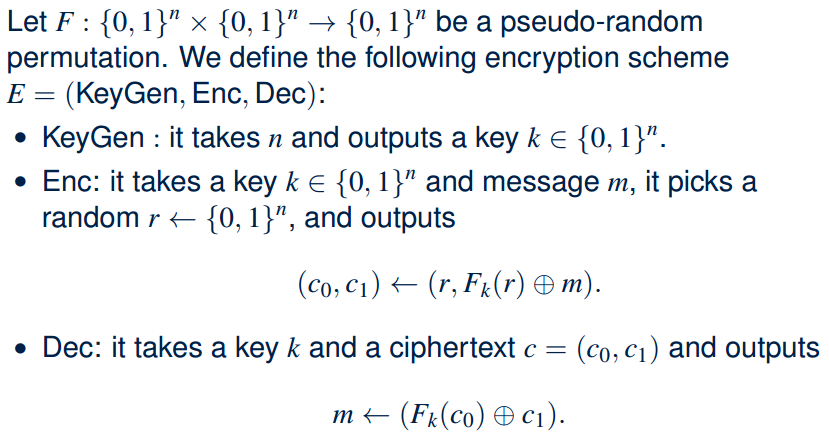
\includegraphics[scale=0.6]{enc-prp}}]~
	\end{description}
	\caption{Encryption with PRP}
	\label{fig:enc-prp}
\end{figure}


\subsection{Symmetric Cryptosystems}
\begin{description}
	\item [{Stream~Ciphers.}] A practical instantiation of a pseudo-random
	generator (PRG) typically with an encryption scheme that uses the
	pseudo-random bits generated by the PRG as the symmetric key to encrypt
	data. Every stream cipher has two main \emph{deterministic} algorithms:
\end{description}
\begin{itemize}
	\item $st_{0}\gets$ Init($s,V$): takes a seed $s$ and an optional initialization
	vector $V$ and outputs an initial state $st_{0}$.
	\item $(y_{i},st_{i})\gets$ GetBits($st_{i}$): takes the $i$-th state
	information $st_{i}$ and outputs a bit $y$ and an updated state
	$st_{i+1}$. 
\end{itemize}
Usually, a \emph{keystream }is produced from the actual key. To encrypt
a bit string $m$ using a pseudo-random bit string $k$, we can compute
$c=m\oplus k$, where $\oplus$ is the bitwise XOR operator. The ciphertext
$c$ can be decrypted using $m=c\oplus k$. 
\begin{description}
	\item [{Authenticated~Encryption~(AE).}] Stream ciphers inherently provide
	no authentication and integrity-protection mechanism. This allows
	an adversary to conduct chosen-ciphertext and malicious bit-flipping
	attacks on the ciphertext. Therefore, a stream cipher is often used
	along message authentication codes (MACs) to protect against such
	attacks (see Figure \ref{fig:ae}). The result is often called an
	authenticated encryption system.
\end{description}
\begin{figure}
	\begin{centering}
		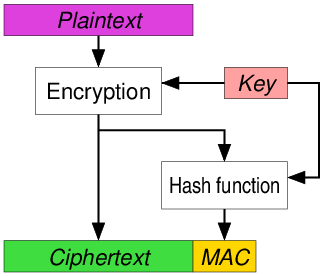
\includegraphics[scale=0.7]{ae}
		\par\end{centering}
	\caption{Authenticated encryption example}
	\label{fig:ae}
\end{figure}

\begin{description}
	\item [{Block~Ciphers.}] A block cipher is a deterministic algorithm for
	encrypting a block of data at once with the same key. AES is a symmetric
	block cipher.
	\item [{Pohlig-Hellman~Cryptosystem.}] Let $p$ be a large prime such
	that $p-1$ has a large prime factor. The Pohlig-Hellman cryptosystem
	is a symmetric cryptosystem, where the key is a pair $x,y\in\mathbb{Z}_{p-1}^{*}$
	such that $xy\bmod(p-1)=1$. A plaintext $m\in\mathbb{Z}_{p}$ is
	encrypted using $c\equiv m^{x}\bmod p$ and a ciphertext is decrypted
	by $m=c^{y}\bmod p$.
	\item [{Deterministic~Encryption.}] A cryptosystem which always generates
	the same ciphertext for a given plaintext and key. Examples are RSA
	and most block ciphers. Deterministic encryption is not semantically-secure
	as it can leak information about the plaintext to an eavesdropper
	if used multiple times; the adversary can simply recognize known ciphertexts
	and learn something every time that ciphertext is transmitted through
	statistical analysis or correlate ciphertexts with user actions.
	\item [{Probabilistic~Encryption.}] A cryptosystem that uses randomness
	in its encryption algorithm and thus produces different ciphertexts
	every time it is called (even with the same plaintext and key). To
	be semantically-secure, an encryption scheme has to be probabilistic.
	Examples of efficient probabilistic encryption algorithms are ElGamal
	and Paillier. A public key encryption scheme most likely needs to
	be probabilistic because the adversary can try encrypting each of
	his guesses under the recipient's public key, and compare each result
	to the target ciphertext.
\end{description}

\subsection{Semantic Security}

\emph{Semantic security} (also called \emph{computational indistinguishability})
guarantees that an adversary who sees the encryption of a message
\textendash{} drawn from a known or chosen message space \textendash{}
gains approximately the same amount of information as it would have
obtained if it did not see the encryption in the first place.
\begin{description}
	\item [{Chosen-Plaintext~Attack~(CPA).}] An adversary enters one or more
	plaintexts (that he has chosen arbitrarily) into the system and obtains
	the resulting ciphertexts. From these pieces of information, he attempts
	to recover the secret key. In CPA, it is like the adversary has access
	to an oracle with the encryption function $\mathsf{Enc}(k,\cdot)$,
	where $k$ is the secret key.
\end{description}
\begin{figure}
	\begin{description}
		\item [{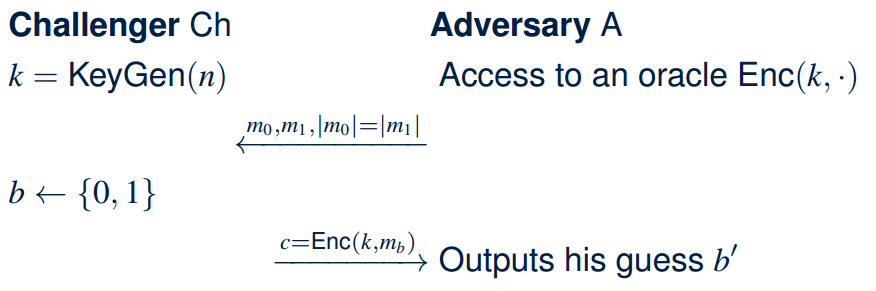
\includegraphics[scale=0.55]{cpa-game}}]~
	\end{description}
	\caption{CPA indistinguishability game}
	\label{fig:cpa-game}
\end{figure}

\begin{description}
	\item [{Chosen-Ciphertext~Attack~(CCA~or~CCA1).}] An adversary enters
	one or more ciphertexts (that he has chosen arbitrarily) into the
	system and obtains the resulting plaintexts. From these pieces of
	information, the adversary attempts to recover the secret key. In
	CCA, it is like the adversary has access to an oracle with the encryption
	function $\mathsf{Enc}(k,\cdot)$ and the decryption function $\mathsf{Dec}(k,\cdot)$,
	where $k$ is the secret key.
\end{description}
\begin{figure}
	\begin{description}
		\item [{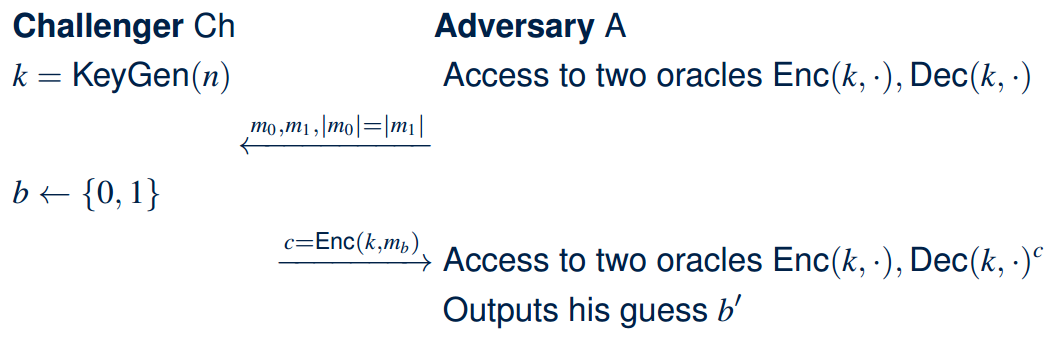
\includegraphics[scale=0.55]{cca-game}}]~
	\end{description}
	\caption{CCA indistinguishability game}
	\label{fig:cca-game}
\end{figure}

\begin{description}
	\item [{Adaptive~Chosen-Ciphertext~Attack~(CCA2).}] An adversary enters
	one or more ciphertexts (that he has chosen arbitrarily) into the
	system and obtains the resulting plaintexts. He then uses these pieces
	of information to choose subsequent ciphertexts that help him recover
	the secret key.
\end{description}

\section{Public Key Cryptography \label{sec:Public-Key-Cryptography}}

A public key encryption scheme acts like a \emph{lock box}. Everyone
is allowed to put something inside a box and lock it, but no one can
open it except those who have the key. In public key encryption, a
message is encrypted (\emph{sealed}) with a \emph{public key} so that
it can only be decrypted using a \emph{secret (private) key.} This
is also known as \emph{asymmetric cryptography} since the scheme requires
two different keys: public key and private key.

If a message $X$ is encrypted with a public key $k$, then anyone
can verify a guess that $Y=X$ by checking whether $\text{Enc}_{k}(Y)=\text{Enc}_{k}(X)$.
This threat is usually eliminated by attaching a large string of random
bits to X before encrypting. Such a random value that is used only
once is called a \emph{nonce}.

\subsection{Diffie-Hellman Key Exchange}
\label{sec:diffie-hellman} In 1976, Diffie and Hellman~\cite{Diffie:2006:NDC:2263321.2269104}
proposed a method for two parties to securely agree on a public key.
This scheme played an important role in the formation of public key
cryptography in 1980s.
\begin{description}
	\item [{DH~algorithm.}] Alice and Bob first agree on a large prime number
	$p$, and a generator (or base) $g$, where $0<g<p$. Alice chooses
	a secret integer $a$ (her private key) and calculates $g^{a}\bmod p$
	(her public key). Bob chooses his private key $b$, and calculates
	his public key in the same way. Alice and Bob then send each other
	their public keys. Alice calculates $(g^{b})^{a}\bmod p=g^{ab}\bmod p$
	and Bob calculates $(g^{a})^{b}\bmod p=g^{ab}\bmod p$. This means
	that they have agreed on a public key $g^{ab}\bmod p$ without learning
	each others private keys $a$ and $b$ unless they can solve the discrete
	logarithm problem, which is computationally infeasible.
	\item [{Security~of~DH.}] The best known algorithm for solving the integer
	factorization problem (and also the discrete logarithm problem) is
	called \emph{General Number Field Sieve (GNFS)}, which has been used
	to break ciphers with a 768-bit long prime $p$. In practice, $p$
	should have at least 1024 bits\footnote{See RFC-3526 for a few parameters used in practice. See RFC-3766 for
		security strength comparison of DH, RSA, and DSA.}. Also, $p-1$ should have a large prime factor $q$, where $g^{q}\bmod p=1$
	(i.e., $q$ be an order of $g$). This secures the algorithm against
	the Pohlig-Hellman attack. The Diffie-Hellman algorithm is vulnerable
	to Man-in-the-Middle attacks unless it is used along with a digital
	signatures scheme to authenticate sender of each message.
	\item [{Elliptic~Curve~Diffie-Hellman~(ECDH).}] Discrete logarithm problem
	(and thus DH algorithm) can be defined over other groups like elliptic
	curves, which result in much smaller key sizes with the same level
	of security. For example 3072-bit DH provides security comparable
	to ECDH-256.
\end{description}

\subsection{RSA Cryptosystem}
\begin{description}
	\item [{Encryption.}] Let $p$ and $q$ be two large primes (say each with
	200 digits) and let $e$ be an integer relatively prime to $(p-1)(q-1)$.
	Also, let $M$ be the message to be encrypted and $n=pq$. The encryption
	of $M$, denoted by $C$, is calculated using 
	\[
	C=M^{e}\bmod n
	\]
	\item [{Decryption.}] Let $d$ be the decryption key, which is an inverse
	of $e$ modulo $(p-1)(q-1)$. The ciphertext $C$ can be decrypted
	using 
	\[
	C^{d}\equiv M\pmod{n}
	\]
	\item [{Security~of~RSA.}] Given $(n,e)$ as the public key, the adversary
	needs to factor $n=pq$ into $p$ and $q$ to compute $(p-1)(q-1)$,
	which can be used to compute the decryption key $d$ from $e$. Hence,
	RSA is secure as long as $n=pq$ cannot be factored in a reasonable
	amount of time, which is currently the case for large $n$'s. This
	is called the \emph{integer factorization problem}. RSA-768 (i.e.,
	RSA with a 768-bit modulus denoted by $n$ above) is the largest RSA
	that is broken so far. RSA-1024 is the most widely-used RSA.
	\item [{Implementation~notes.}] The large primes $p$ and $q$ can be
	found efficiently using a \emph{primality test} algorithm. The encryption
	can be performed using a fast \emph{modular exponentiation} algorithm.
\end{description}

\subsection{ElGamal Cryptosystem}

The Diffie-Hellman key exchange protocol~\cite{Diffie:2006:NDC:2263321.2269104}
is can be used for generating shared secrets (usually used as crypto
keys for encryption algorithms), but it cannot be used directly for
encryption itself. The simplest way to use Diffie-Hellman as part
of an encryption algorithm is to generate a shared one-time-pad that
is XOR'd with the plaintext. The ElGamal encryption algorithm does
basically this, the only difference is that it uses modular multiplication
instead of XOR'ing to do the encryption once it has the shared one-time-pad.
ElGamal cryptosystem is semantically-secure under CPA, but is not
semantically-secure under CCA. For applications where CCA security
is important one may use a CCA-secure cryptosystem such as Crame-Shoup
\cite{Cramer:1998:PPK:646763.706340}. 

Let $p$ be a large prime such that $p-1$ has a large prime factor
$q$. Let $g\in\mathbb{Z}_{p}^{*}$ be an element of order $q$ in
$\mathbb{Z}_{p}^{*}$. In the ElGamal scheme, the private key is $x\in\{0,...,q-1\}$
and the public key is $g^{x}\bmod p$. A plaintext $m\in\mathbb{Z}_{p}$
is encrypted by the pair $(g^{y}\bmod p,m\cdot g^{xy}\bmod p)$, where
$y\in\{0,...,q-1\}$ is a per-round (fresh) random value. 

The ElGamal and the Pohlig-Hellman cryptosystems are \emph{mutually
	commutative} meaning that a ciphertext encrypted under multiple ElGamal
keys, multiple Pohlig-Hellman keys, or any mixture of the keys can
be decrypted by the set of decryption keys in any order.

\subsection{Distributed Key Generation}

Distributed key generation (DKG) allows a set of $n$ parties to jointly
generate a pair of public and private keys in a such a way that the
public key is output in the clear while the private key is shared
by the parties via a threshold secret-sharing scheme such as that
of \cite{shamir:how}. For discrete-log based threshold schemes, distributed
key generation means a distributed generation (i.e., without a trusted
dealer) of a Shamir secret sharing \cite{shamir:how} of a random
value $x$ as the private key, and $y=g^{x}$ as the public key.

Pedersen~\cite{pedersen1991threshold} proposed a simple and efficient
DKG protocol that was later shown by Gennaro et al.~\cite{Gennaro1999}
as failing to generate the private key (and the public key) with uniform
distribution. They show that an adversary who compromises even two
out of $n$ parties can skew the distribution of the generated secret
key. They also propose a new DKG protocol that fixes this problem
by generating the private key with a uniform distribution. While Pedersen\textquoteright s
protocol is non-interactive in the absence of faults, the protocol
of Gennaro et al. requires two rounds of communication.

In a later work, Gennaro et al.~\cite{Gennaro03revisitingthe} show
that a certain type of discrete-log based threshold schemes can remain
secure even if they use Pedersen\textquoteright s DKG protocol as
a subprotocol. Namely, they show how to prove secure a threshold version
of Schnorr\textquoteright s signature scheme~\cite{Schnorr:1989:EIS:646754.705037}
instantiated with Pedersen\textquoteright s DKG protocol.

\subsection{Verifiable Random Functions}

First introduced by Micali, Rabin, and Vadhan in 1999~\cite{micali:1999:vrf},
a VRF is a pseudorandom function (PRF), where the party holding the
secret key can produce a non-interactive proof that the function was
evaluated correctly. The initial construction was inefficient. Dodis
and Yampolskiy~\cite{dodis:yampolskiy:2005} propose an efficient VRF construction
using bilinear maps.

\subsection{Miscellaneous }
\begin{description}
	\item [{Threshold~Cryptography.}] In threshold cryptography, the message
	is encrypted using a public key and the corresponding secret key is
	shared among $n$ parties. To decrypt the message, at least $t$ parties
	are required to cooperate in the decryption algorithm. Such a scheme
	is called a $(t,n)$-threshold cryptosystem.
	\item [{Anonymous~Public-Key~Encryption/Signatures.}] Encrypt/sign a
	message for reading/verifying by any member of an explicit anonymity
	set. For example, a group can use this to perform anonymous group
	communication, or a member of an organization's board of trustees
	might prove to be a member of the board without revealing which member
	he is (\emph{anonymous authentication}). If the provided anonymity
	set contains only one public key, this reduces to conventional single-receiver
	public-key encryption/signatures.
\end{description}

\section{Message Authentication and Integrity \label{sec:commitment-schemes}}

Message authentication schemes guarantee that a message is sent by
a valid sender. Message integrity schemes ensure that a message is
protected from being manipulated or modified by an adversary. Confidentiality
schemes (e.g. encryption and secret sharing) do not necessarily provide
message integrity.

\subsection{Message Authentication Codes}

In order to verify integrity and authenticity of a message, an additional
piece of information called MAC is generated using a MAC algorithm
and sent along with the message to the receiver. The receiver then
generates the MAC from the received message using the same MAC algorithm
and verifies that both MACs match. This prevents the adversary from
manipulating the messages. 

The MAC algorithm requires a \emph{MAC key} along with the message
to generate the MAC. This method assumes the sender and receiver have
the same MAC key as in the case of symmetric encryption. This is the
difference between MACs and digital signatures as the latter is based
on asymmetric encryption and provides \emph{non-repudiation}, meaning
that it proves that a message was signed by no one other than that
holder of the secret key (i.e., its private key).

\subsection{Digital Signatures}

Digital signature (DS) algorithms are used to provide message authentication
and integrity. A DS algorithm is usually based on public-key (asymmetric)
cryptosystems (Section~\ref{sec:Public-Key-Cryptography}) and thus,
usually consists of three algorithms 
\begin{itemize}
	\item $(pk,sk)=\mathsf{Keygen}()$
	\item $s=\mathsf{Sign(}m,sk\mathsf{)}$
	\item $\mathsf{Verify(}m,s,pk\mathsf{)}$,
\end{itemize}
where $m$ is the message to be signed, $s$ is the signature, and
$pk$ and $sk$ are the public key and the secret key respectively
generated by $\mathsf{Keygen}$.\textsf{ }If a message is digitally-signed
via $\mathsf{Sign}$, then $\mathsf{Verify}$ fails if and only if
\begin{itemize}
	\item the message is changed after signing, and/or
	\item the message is signed with an invalid secret key (i.e., the secret
	key does not belong to the person the sender claims to be).
\end{itemize}
The idea behind DS schemes is to use a one-way function (Section~\ref{sec:One-Way-Functions}):
a message can be signed by computing the inverse of a one-way function
using the secret key, and the signature can be verified by computing
the forward direction. However, this type of DS is not semantically-secure
because the adversary can use $\mathsf{Verify}$ to find a valid pair
of a message and a signature.
\begin{description}
	\item [{Non-Repudiation.}] A \emph{non-repudiable (non-transferable) signature}
	is a signature that is uniquely bound to the identity of the signer.
	Therefore, the signer cannot deny later that it signed the message.
	Non-repudiation can be achieved using public key cryptosystems. Singing
	a message using a symmetric encryption scheme such as a MAC does not
	provide non-repudiation because if Bob receives a message from Alice
	encrypted with a secret that is shared only between them, then Bob
	cannot prove to other parties that the message came from Alice. This
	is because there is no way to prove it was Alice and not Bob who signed
	the message with the shared secret. Such a signature is called a \emph{transferable
		signature}.
\end{description}

\subsubsection{Public-Key Authentication}

A client proves its control of a private key associated with a public
key by performing an operation which requires knowledge of the private
key. This works by sending a signature created with the private key
of the user. The signature is then verified using the public key of
the user. Any public key algorithm may be offered for use in this
type of authentication. 

In SSH (see Figure~\ref{fig:SSH-Auth}), the user authentication
protocol starts by the server sending a random challenge message $M$
to the client. Then, the client encrypts $M$ with its private key
and sends it to the server. Finally, the server decrypts the message
with the user's public key and if the result matches $M$, it sends
a success message to the client. See \cite{rfc4252} for more details
about SSH public-key authentication.

\begin{figure}
	\begin{description}
		\item [{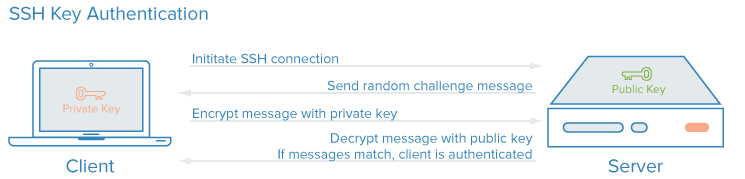
\includegraphics[scale=0.7]{ssh-auth}}]~
	\end{description}
	\caption{Public-key authentication in SSH.}
	\label{fig:SSH-Auth}
\end{figure}


\subsection{Commitment Schemes }

In a commitment scheme, a party commits to a secret value so that
other parties ensure that he cannot change the value after he has
committed to that value (called \emph{consistency verification}).
Every commitment scheme consists of two phases: 
\begin{enumerate}
	\item \textbf{Commit phase.} The sender sends a \emph{commitment message}
	along with the secret to the receiver while ensuring, 
	\begin{itemize}
		\item The commitment message reveals nothing to the receiver (\emph{hiding
			property}), 
		\item The commitment message is the only possible commitment value that
		the sender can compute from the message (\emph{binding property}). 
	\end{itemize}
	\item \textbf{Reveal phase.} The receiver wants to \emph{open} (i.e., check)
	the commitment. The sender sends an \emph{opening message} to the
	receiver, with which the receiver can perform a \emph{check} that
	verifies consistency. 
\end{enumerate}
In other words, the commitment $C$ to the value $x$ is computed
as $C=\mathsf{Commit}(x,open)$, where $open$ is a random value that
is also sent in the reveal phase as the opening message. The receiver
then verifies the commitment using $\mathsf{CheckReveal}(C,x,open)$.

A commitment scheme is \emph{perfectly-hiding} (\emph{perfectly-binding})
if no unbounded adversary can break the hiding (binding) property
described above. A commitment scheme is \emph{computationally-hiding}
(\emph{computationally-binding}) if no polynomial-time adversary can
break the hiding (binding) property. In general, a scheme cannot be
both perfectly-hiding and perfectly-binding, because they are opposing
principles.

A commitment scheme is \emph{statistically-hiding} if the receiver
can obtain some advantage from the commitment message but this advantage
is provably exponentially small in the security parameter. Note that
the receiver can still be unbounded in this type of commitment scheme.

Hiding property of commitment schemes is more crucial in some applications
like verifiable secret sharing because it guarantees secrecy of the
inputs. Binding property guarantees consistency, which is less critical
than secrecy. For example in VSS, consistency violation at most results
in incorrect sharing (or incorrect computation result in multiparty
computation), which is more tolerable than revealing information about
the secrets. Feldman~\cite{Feldman:1987:PSN:1382440.1383000} introduces
several commitment schemes all of which are computationally-binding
and computationally-hiding. On the other hand, \cite{Pedersen:1991:NIS:646756.705507}
gives a computationally-binding but perfectly-hiding commitment scheme,
which can be used in unconditional models where the dealer is polynomial-time.

\subsubsection{Pedersen Commitment Scheme}

Pedersen~\cite{Pedersen:1991:NIS:646756.705507} proposes a perfectly-hiding
and computationally-binding commitment scheme\footnote{Pedersen proposes his commitment scheme as a part of a verifiable
	secret sharing scheme (see section~\ref{sec:vss}), which uses the
	commitment scheme to verify consistency of shares in Shamir's secret
	sharing scheme~\cite{shamir:how}. Obviously, such a commitment scheme
	can be generally used in other applications like digital signatures
	and zero-knowledge proofs.}, which is based on the difficulty of solving the discrete logarithm
problem. Let $p$ and $q$ be primes such that $q$ divides $p-1$
and let $\mathbb{Z}_{q}$ be the additive group of integers modulo
$q$ and $\mathbb{Z}_{p}^{*}$ be the multiplicative group of integers
modulo $p$. To commit to a value $s\in\mathbb{Z}_{q}$, the sender
chooses $r\in\mathbb{Z}_{q}$ uniformly at random and computes the
commitment 
\[
C(s,r)=g^{s}h^{r},
\]
where $g,h\in\mathbb{Z}_{p}^{*}$. The commitment can be opened (and
then checked) once $s$ and $r$ are revealed. This scheme has the
following homomorphic property 
\[
C(s_{1},r_{1})\cdot C(s_{2},r_{2})=C(s_{1}+s_{2},r_{1}+r_{2}).
\]


\subsection{Anonymous Credentials}

Anonymous credentials, first introduced by Chaum~\cite{Chaum:1985:SWI:4372.4373},
provide a mechanism for users of a system to anonymously prove assertions
about themselves by issuing cryptographic credentials (or tokens)
without disclosing any information but the fact that he possesses
a valid credential. For example, an anonymous credential can be used
to anonymously authenticate a user (i.e., prove his membership to
an organization without revealing his identity) or to prove an assertion
about the user in a privacy-preserving manner such as proving that
the user is 18+ years old without revealing his exact date of birth.

It should be impossible (or practically hard) for an adversary to
forge a credential for a user or link different credentials of the
same user to each other when the user is assigned multiple credentials
in different transactions. If the same credential can be used in multiple
transactions, then it is called a \textit{multiple-show credential}.
Otherwise, it is called a \textit{one-show credential.} In order to
make multiple transactions unlinkable for a one-show credential, a
set of credentials is issued and for each anonymous transaction, a
new credential is used.

Anonymous credential systems are closely related to \textit{blind
	signatures}\emph{~}\cite{Chaum1983}, zero-knowledge proofs, and
\textit{group signatures}\emph{~}\textit{\cite{Ateniese2000}} (escrow
schemes). In the latter, a group member signs messages anonymously
on behalf of the group.

\subsubsection{Blind Signatures}

In some applications such as e-voting systems and cryptocurrency,
the signer and the author of a message are different parties, and
the author does not want the signer to see the content of his message.
Blind signatures\emph{~}\cite{Chaum1983} allow the content of a
message to be encrypted (blinded) before it is signed. The resulting
signature can then be publicly verified against the original message.

\subsubsection{Ring Signatures}

Introduced by Rivest, Shamir, and Tauman\emph{~}\cite{Rivest2001},
a \emph{ring signature} can provide an anonymous signature from a
member of a group without revealing which member signed the message.
This is useful for whistleblowing, as hinted by the title \emph{How
	to leak a secret} of \cite{Rivest2001}. A group of parties each have
public/private key pairs $(PK_{1},SK_{1}),(PK_{2},SK_{2}),...,(PK_{n},SK_{n})$.
Party $i$ can compute a ring signature $\sigma$ on a message $m$,
on input $(m,SK_{i},PK_{1},...,PK_{n})$. Anyone can check the validity
of the signature given $\sigma$, $m$, and $PK_{1},...,PK_{n}$.
The anonymity property is that any verifier should not have a probability
greater than $1/n$ to guess the identity of the real signer who has
computed a ring signature.
\begin{description}
	\item [{Linkable~Ring~Signatures.}] Introduced by Liu~et~al.~\cite{Liu2004},
	an LRS scheme allows anyone to determine whether two ring signatures
	are signed by the same group member without disclosing the identity
	of the member. This allows a verifier to check distinctness and prevent
	the signer from signing or authenticating himself more than once and
	thus preventing Sybil attacks~\cite{douceur02sybil} and double-voting
	in e-voting systems. The algorithm of \cite{Liu2004} makes $O(n)$-long
	signatures, where $n$ is the group size. Au et al.~\cite{Au2006}
	propose a constant-size LRS algorithm.
\end{description}

\section{Interactive Proofs }

An \emph{interactive proof} is a conversation between a prover and
a verifier that ends with the verifier either accepting or rejecting
the prover's statement. The prover and the verifier exchange \emph{challenges}
and \emph{responses}, typically dependent on random numbers that they
are allowed to keep secret. Interactive proofs used for identification
may be formulated as proofs of knowledge. In this scenario, Alice
has a secret $s$, and she wishes to convince Bob that he has knowledge
of $s$ by responding correctly to queries made by Bob that require
knowledge of $s$ to answer.

An interactive proof is called to be a \emph{proof of knowledge (PoK)
}if it provides two properties: \emph{soundness} and \emph{completeness:}
\begin{itemize}
	\item \textbf{Completeness:} An interactive proof protocol is \emph{complete}
	if, given an honest prover and an honest verifier, the protocol succeeds
	with overwhelming probability (i.e., the verifier accepts the prover\textquoteright s
	claim).
\end{itemize}
Informally, completeness means that the protocol is correct for honest
prover and honest verifier.
\begin{itemize}
	\item \textbf{Soundness: }An interactive proof protocol is \emph{sound}
	if there exists an expected polynomial time algorithm that if a dishonest
	prover can with non-negligible probability execute the protocol with
	the verifier, then the algorithm can be used to extract the knowledge
	from the prover.
\end{itemize}
Informally, soundness means the protocol is secure against a dishonest
prover. In other words, a malicious prover cannot convince an honest
verifier to accept the prover's statement unless the prover knows
some secret.

\paragraph{$\Sigma$-protocol. \textmd{PoK protocols often consist of three
		rounds: commitment, challenge, and response. Such a protocol is called
		a $\Sigma$-protocol}~\cite{sigma:protocols:damgard}.}

\subsection{Zero-Knowledge Proofs}

First introduced by Goldwasser, Micali, and Rackoff~\cite{Goldwasser:1985:KCI},
a zero-knowledge protocol allows PoK without revealing the an information
about the knowledge to a (polynomial-time) adversary. To define the
zero-knowledge property, we need to first define two concepts:

\paragraph{View. \textmd{A view (or transcript) of a PoK is the sequence of
		steps taken between the prover and the verifier in the PoK.}}

\paragraph{Simulator. \textmd{A simulator is a procedure that can generate fake
		views that are indistinguishable from the original view of the PoK
		generated with the prover.}}

\paragraph{Zero-Knowledge~Proof. \textmd{A zero-knowledge proof (ZKP) is a
		proof of knowledge that can additionally provide the following property:}}
\begin{itemize}
	\item \textbf{Zero-Knowledge: }A PoK has the zero-knowedge property if there
	exists a simulator for the proof.
\end{itemize}
Informally, this means that no amount of knowledge should pass between
the prover and the verifier that the verifier could not figure out
without the help of the prover. In other words, if an adversary can
successfully verify the proof after communicating with the prover,
then the adversary could just as well have succeeded without the prover
by just running the simulator. This guarantees that the number of
times that the prover participates in them does not vary the chances
of success of impersonation attacks.

\subsubsection{Non-Interactive Zero-Knowledge Proof}

\paragraph{\textmd{If the proof is done with no interaction between the prover
		and the verifier, then it is called a }\textmd{\emph{non-interactive
			zero-knowledge proof (NIZK)}}\textmd{. Goldreich and Oren \cite{goldreich1994}
		show that NIZK is impossible in the standard model meaning that some
		assumption like a common reference string (CRS) or a random oracle
		are needed. Using the Fiat-Shamir heuristic \cite{fiat1986prove}, one
		can construct a NIZK protocol in the random oracle model from an interactive
		ZK protocol. }}

\paragraph{zk-SNARK.\textmd{ A }\textmd{\emph{zero-knowledge succinct non-interactive
			argument of knowledge (zk-SNARK)}}\textmd{ allows a constant-size
		ZKP in terms of the size of the circuit representing the program that
		its correct execution is being verified. The program is compiled into
		an equation of polynomials $t(x)\cdot h(x)=w(x)\cdot v(x)$, where
		the equality holds if and only if the program is computed correctly.
		The prover wants to convince the verifier that this equality holds.
		To reduce the proof size and the verification time, the verifier chooses
		a secret evaluation point $s$ to reduce the problem from multiplying
		polynomials and verifying their equality to multiplication and equality
		check on numbers: $t(s)\cdot h(s)=w(s)\cdot v(s)$.}}

A (partially) homomorphic encryption function $E$ is used so that
the prover can compute $E(t(s)),E(h(s)),E(w(s)),E(v(s))$ from $E(s)$
without knowing $s$. A zk-SNARK requires a trusted setup which generates
a common reference string (CRS) for the NIZK. In this setup, the verifier
chooses a random and secret field element $s$ and encrypts the values
of the polynomials at that point.

\subsection{Proof of Discrete Logarithm}

Chaum et al.\ \cite{Chaum:87:ZKP} propose a protocol for proving
the knowledge of a discrete logarithm. Figure~\ref{fig:CEG-ZKP}
shows the protocol rounds. In this protocol, Alice (the prover) wants
to prove to Bob (the verifier) that she knows the discrete logarithm
of $g^{x}\bmod p$, which is $x$.

\begin{figure}
	\begin{description}
		\item [{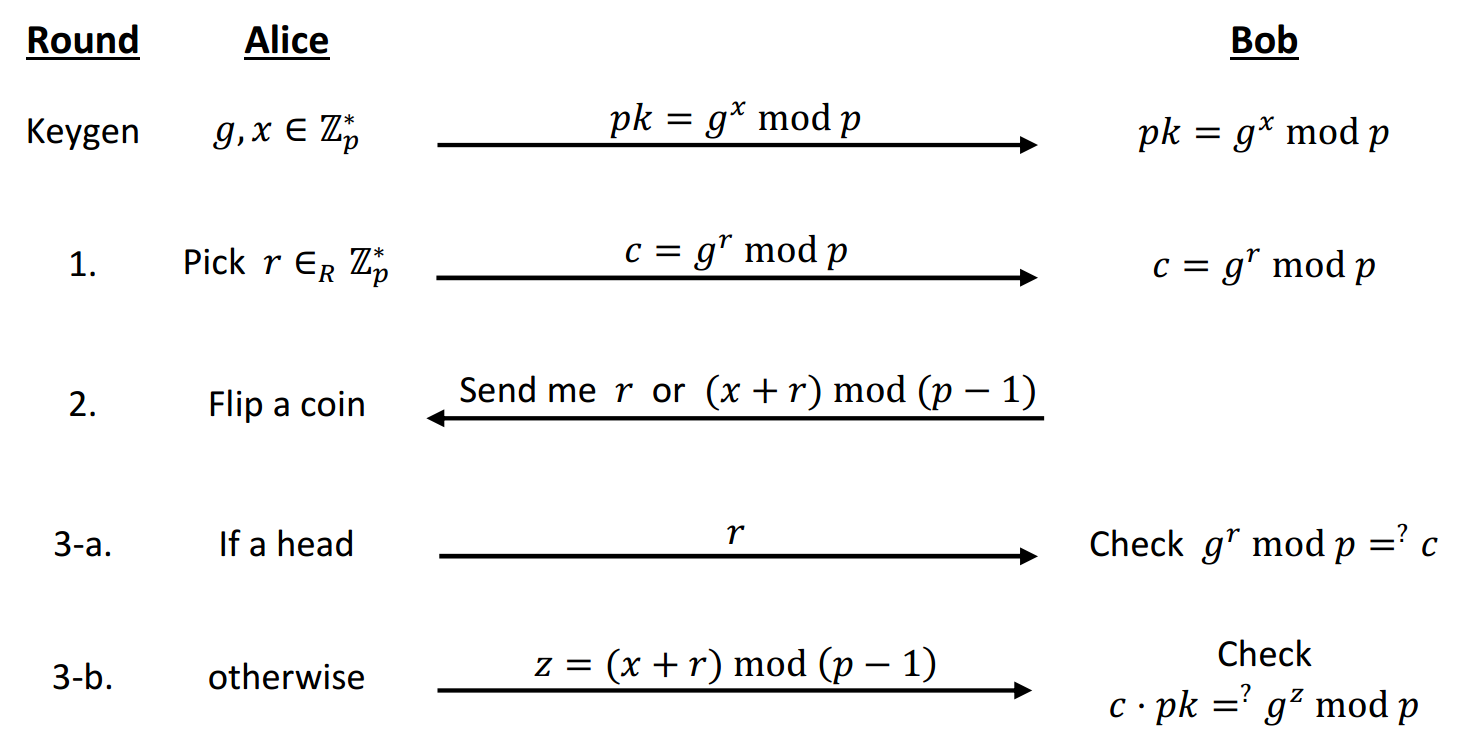
\includegraphics[scale=0.5]{cev-zkp}}]~
	\end{description}
	\caption{Proof of knowledge of discrete log \cite{Chaum:87:ZKP}.}
	\label{fig:CEG-ZKP}
\end{figure}


\section{Elliptic Curve Cryptography}

The goal of Elliptic Curve Cryptography (ECC) is to provide the same
level of security as RSA or discrete logarithm systems but with significantly
shorter keys (about 160-256 bit vs. 1024-3072 bit). ECC is based on
the discrete logarithm problem defined on elliptic curve groups. There
is no known efficient discrete-logarithm solving algorithm for elliptic
curves, beyond the generic algorithms, which work on every group.
\begin{description}
	\item [{Elliptic~Curve.}] An elliptic curve is a set of points $(x,y)$
	defined by any equation in the form 
	\[
	y^{2}=x^{3}+ax+b.
	\]
	In cryptography, such a curve is defined over finite fields rather
	than real numbers, i.e., for a prime $p$ an elliptic curve over $\mathbb{Z}_{p}$
	is defined using 
	\[
	y^{2}\equiv x^{3}+ax+b\bmod{p},
	\]
	where $a,b\in\mathbb{Z}_{p}$. This curve must be \emph{nonsingular}
	meaning that it must not intersect itself. Algebraically, this means
	that the discriminant $\Delta=-16(4a^{3}+27b^{2})$ is nonzero.
\end{description}
The points on an elliptic curve and a \emph{point at infinity} form
a group under a certain addition law. If $P$ and $Q$ are two points
on the curve, then the addition law defines a unique third point,
$P+Q$. A \emph{primitive point} $G$ is a \emph{generator} of this
group: all elements of the group can be generated as $G+G+\cdots+G$
($k$ times) for some $k$.

\subsection{Elliptic Curve Diffie-Hellman}

To generate a pair of private/public keys over an elliptic curve such
that finding the private key from the public key is as hard as solving
the discrete-logarithm problem, one chooses a pseudorandom scalar
value $x$ as his private key using a PRG. Then, he sets $x\times G$
as his public key, where $G$ is a generator of an elliptic curve,
and $\times$ denotes elliptic curve point multiplication by a scalar.

Let $(a,a\times G$) and $(b,b\times G)$ be Alice and Bob's public/private
key pairs. Alice sends $a\times G$ to Bob, and Bob sends $b\times G$
to Alice. Alice computes the shared secret using $a\times(b\times G)$
and Bob computes $b\times(a\times G)$. Since the $a\times(b\times G)=b\times(a\times G)$,
the parties have agreed on the same secret.

\subsection{Elliptic Curve Digital Signature}

Let $G$ be a generator of an elliptic curve with large prime order
$n$. Also, let $(x,Q_{A})$ be Alice's private key/public key such
that $Q_{A}=x\times G$. To sign a message $m$ using her private
key $x$, Alice performs the following steps:
\begin{enumerate}
	\item Calculate $e=H(m)$, where $H$ is a cryptographic hash function such
	as SHA-2;
	\item Choose a random integer $k$ from $[1,n-1]$;
	\item Calculate the point $(x_{1},y_{1})=k\times G$ on the elliptic curve;
	\item Calculate $r=x_{1}\mod n$. If $r=0$, then go to step 2;
	\item Calculate $s=k^{-1}(e+r\cdot x)\mod n$. If $s=0$, then go to step
	2;
	\item The signature is $(r,s)$.
\end{enumerate}
To verify a signature, Bob performs the following steps:
\begin{enumerate}
	\item Verify that $r$ and $s$ are integers in $[1,n-1]$;
	\item Calculate $e=H(m)$;
	\item Calculate $w=s^{-1}\mod n$;
	\item Calculate $u_{1}=zw\mod n$ and $u_{2}=rw\mod n$;
	\item Calculate the point $(x_{1},y_{1})=u_{1}\times G+u_{2}\times Q_{A}$;
	\item The signature is valid if and only if $r=x_{1}\mod n$.
	\item $a\times H_{3}(h)-a\times H_{3}(h)$
\end{enumerate}

\section{Homomorphic Encryption}

Homomorphic encryption is a form of encryption, which allows specific
types of computations to be carried out on ciphertext and obtain an
encrypted result which decrypted matches the result of operations
performed on the plaintext. More formally, in homomorphic encryption
we define a function $f$ such that $f(x)=d(f(e(x)))$, where $x$
is the plaintext, $e(x)$ is the encryption function and $d(x)$ is
the decryption function. We call $f$ a homomorphic function. Although
a cryptosystem which is unintentionally homomorphic can be subject
to attacks, if treated carefully, homomorphism can be used to perform
secure computations.

An encryption scheme is called \emph{additive homomorphic} if it is
possible to compute an encryption of $(m_{1}+m_{2})$ from the encryptions
of $m_{1}$ and $m_{2}$. This operation is called homomorphic addition
and is denoted by $+_{h}:E(m_{1}+m_{2})=E(m_{1})+_{h}E(m_{2})$. Different
cryptosystems support different levels of homomorphism. \textit{Partially
	homomorphic encryption (PHE)} methods allow homomorphic encryption
of either addition or multiplication on plaintexts. Table~\ref{tab:partial-he}
lists various PHE methods.

\begin{table}[H]
	\caption{Homomorphic properties of various cryptosystems}
	\label{tab:partial-he}
	\centering{}\vspace{7pt}
	%
	\begin{tabular}{l|l}
		\hline 
		\textbf{Cryptosystem } & \textbf{Homomorphic operations }\tabularnewline
		\hline 
		RSA~\cite{Rivest:1978:MOD:359340.359342}  & Multiplication\tabularnewline
		Goldwasser-Micali~\cite{Goldwasser:1982:PEA:800070.802212}  & XOR \tabularnewline
		ElGamal~\cite{ElGamal:1985:PKC:19478.19480}  & Multiplication, Exponentiation by constant\tabularnewline
		Benaloh~\cite{Benaloh94denseprobabilistic}  & Addition \tabularnewline
		Paillier~\cite{Paillier:1999:PCB:1756123.1756146}  & Addition, Multiplication by constant \tabularnewline
		\hline 
	\end{tabular} 
\end{table}


\subsection{Fully Homomorphic Encryption}

A cryptosystem which supports both addition and multiplication is
called \textit{fully homomorphic encryption (FHE)}. Such a system
also preserves the useful algebraic properties of a ring. Using an
FHE scheme, any circuit can be homomorphically evaluated. There are
several efficient PHE methods but research on efficient FHE schemes
is still ongoing.

An FHE scheme allows to perform \emph{non-interactive secure computation},
which is very useful in the applications that permit small number
of interactions between parties. The first FHE scheme was proposed
by Craig Gentry in 2009~\cite{Gentry:2009:FHE:1536414.1536440},
which is based on lattices and is very computationally intensive.
However, in the past four years the efficiency of lattice-based FHE
schemes has been improved by several orders of magnitude giving some
hope to the community. The ciphertexts in all these schemes are \emph{noisy},
with a noise that grows slightly during homomorphic addition, and
explosively during homomorphic multiplication.
\begin{description}
	\item [{Somewhat~Homomorphic~Encryption~(SHE).}] Current FHE schemes
	can only evaluate small circuits due to some noise term. In other
	words, they allow homomorphic operations to be performed only a limited
	number of times because the error term increases with each operation.
	Once the error exceeds a certain tolerance, the result can no longer
	be decrypted.
	\item [{Bootstrapping.}] Gentry~\cite{Gentry:2009:FHE:1536414.1536440}
	starts with an SHE scheme and then shows how to make it bootstrappable.
	An SHE scheme is \emph{bootstrappable} if it can decrypt messages
	with a sufficiently small error constant. In other words, it implements
	a \texttt{Recrypt} function which \emph{refreshes} the ciphertext
	by homomorphically decrypting and then re-encrypting the message,
	which reduces the error term. Using the bootstrapping procedure, we
	can perform unlimited number of homomorphic operations and hence,
	we get an FHE scheme from an SHE scheme.
\end{description}

\section{Pairing-Based Cryptography}

Let $G_{1}$ and $G_{2}$ be additive groups and $G_{T}$ be a multiplicative
group, all of prime order $p$. Also, let $g_{1}\in G_{1}$ and $g_{2}\in G_{2}$
be generators of $G_{1}$ and $G_{2}$ respectively. We define a \emph{bilinear
	pairing} (or a \emph{bilinear map}) to be the map $e:G_{1}\times G_{2}\to G_{T}$
such that 
\[
e(ag_{1},bg_{2})=e(g_{1},g_{2})^{ab},
\]
for all $a,b\in\mathbb{Z}_{p}$ and $e(g_{1},g_{2})\neq1$. Clearly,
if $G_{1}$ and $G_{2}$ are multiplicative groups, then the bilinearity
property becomes 
\[
e(g_{1}^{a},g_{2}^{b})=e(g_{1},g_{2})^{ab}.
\]
In practice, the pairing $e$ is required to be efficiently computable.
In some applications, the pairing is also required to be hard to invert.

\subsection{The BLS Signature Scheme}

Boneh, Lynn, and Sacham~\cite{Boneh:2001:SSW:647097.717005} propose
a pairing-based\emph{ }digital signature scheme that is secure in
the random-oracle model. The scheme generates short signatures that
are elements of an elliptic curve group and uses the Weil bilinear
pairing to verify the signatures.
\begin{description}
	\item [{Key~Generation.}] All parties agree on three groups $G_{1}$,
	$G_{2}$, and $G_{T}$ of prime order $p$ and a generator $g$ of
	$G_{2}$. Each party chooses a random integer $x\in[0,p-1]$ as its
	private key and broadcasts $g^{x}$ as the public key.
	\item [{Signing.}] To sign a message $m$, first take a hash of the message
	$h=H(m)\in G_{1}$, and then compute the signature $h^{x}\in G_{1}$.
	\item [{Verification.}] Let $e:G_{1}\times G_{2}\to G_{T}$ be a bilinear
	pairing. Given the signature $h^{x}$, the public key $g^{x}$, and
	the message $m$, verify that $e(h^{x},g)=e(H(m),g^{x})$.
\end{description}
Correctness can be simply proved using the bilinearity property $e(h^{x},g)=e(h,g^{x})$.

\section{Identity-Based Encryption}

In public-key encryption, if a party $P$ wants to send encrypted
messages $m_{1},...,m_{n}$ to $P_{1},...,P_{n}$, he needs to know
public keys $PK_{1},...,PK_{n}$ of the recipients so that he sends
$c_{i}=\mathsf{Enc}(PK_{i},m_{i})$ to $P_{i}$ who can decrypt $m_{i}=\mathsf{Dec}(SK_{i},c_{i})$
with his own secret key $SK_{i}$. Due to the nature of the encryption
scheme, public keys are usually long and obtaining them adds a communication
overhead. In practice, each recipient often holds an identity that
can usually be represented with a much shorter bit string and is independent
of the encryption scheme.

In \emph{identity-based encryption (IBE)}, the key generation protocol
only generates a single public key that can be used along with the
identity of each recipient to encrypt the corresponding recipient's
message. In other words, party $P$ encrypts $m_{i}$ for party $P_{i}$
using $c_{i}=\mathsf{Enc}(PK,ID_{i},m_{i})$, where $PK$ is the common
public key and $ID_{i}$ is the identity of $P_{i}$.

The key generation protocol also generates a master secret key $MSK$
which is used by each recipient $P_{i}$ along with the recipient's
identity $ID_{i}$ to generate $P_{i}$'s own secret key using $SK_{i}=\mathsf{Extract}(MSK,ID_{i})$.
Using this secret key, $P_{i}$ decrypts his cipher using $m_{i}=\mathsf{Dec}(SK_{i},c_{i})$.
Therefore, an IBE scheme provides four functionalities: $\mathsf{Setup}$,
$\mathsf{Extract}$, $\mathsf{Enc}$, and $\mathsf{Dec}$. The most
well-known IBE scheme is due to Boneh and Franklin~\cite{Boneh2001ibe}
which is based on bilinear maps and is shown secure under bilinear
Diffie-Hellman (BDH) assumption.

\section{Distributed Consensus}

One of the most fundamental problems in distributed computing happens
when a group of parties want to agree on a common value without the
help of any trusted third party while some of the parties are being
controlled by an adversary. When the faulty behavior is limited to
crash failures (a.k.a., fail-stop) but corrupt parties otherwise follow
the protocol, this problem is known as\emph{ distributed consensus.
}If the parties can deviate arbitrary from the protocol (i.e., are
Byzantine), then this problem is known as \emph{Byzantine agreement.}

The impossibility result of \cite{FLP} shows that deterministic asynchronous
consensus protocols cannot guarantee protocol termination. Therefore,
in many cases, we rely on probabilistic (randomized) protocols to
achieve agreement with all but negligible probability. In the following
section, we describe the Byzantine agreement problem and state known
important results.

\subsection{Byzantine Agreement}

In 1982, Lamport, Shostak, and Pease \cite{lsp82} were the first
to introduce the problem of Byzantine Generals as follows: 
\begin{quote}
	``...a group of generals of the Byzantine army camped with their
	troops around an enemy city. Communicating only by messenger, the
	generals must agree upon a common battle plan. However, one or more
	of them may be traitors who will try to confuse the others. The problem
	is to find an algorithm to ensure that the loyal generals will reach
	agreement.''
\end{quote}
\begin{description}
	\item [{Problem~Statement.}] Consider $n$ parties, of which up to $t$
	may be corrupted by an adversary and exhibit arbitrary faults; the
	remaining parties are honest. Every party starts out with an initial
	value and the goal is to agree on a common value that is equal to
	some honest party's input. For example, if all parties start with
	1, they must all decide on 1.
\end{description}
Let $t$ be the number of corrupted parties. The following important
results about Byzantine agreement (BA) exists in the literature:
\begin{itemize}
	\item For $t<n/3$, BA is possible using a deterministic protocol with round
	complexity $O(t)$ \cite{pease80reaching} and using a probabilistic
	protocol with expected round complexity $O(1)$ \cite{Feldman:1988:OAB:62212.62225}.
	\item For $t<n/2$, BA is possible with cryptographic assumptions, e.g.,
	a public-key infrastructure (PKI) \cite{pease80reaching}.
\end{itemize}
With the assumption of private channels, Feldman and Micali~\cite{feldman}
propose a randomized BA protocol with constant expected time. Later,
Canetti and Rabin~\cite{canetti:rabin:1993:ba} achieved the optimal resiliency
bound of $t<n/3$ for asynchronous BA with private channels. With
cryptographic assumptions, Cachin~et~al.~\cite{cachin00randomoracles}
achieve constant communication and polynomial computation complexities
in the asynchronous model with adaptive adversary. 

In the full information model, Kapron~et~al.~\cite{kapron:2008} propose
a polylogarithmic BA assuming the adversary is static. Their protocol
elects a logarithmic subset of parties less than $1/3$ of which are
corrupted with high probability. When the adversary is adaptive, the
best known BA protocol in the full information model has expected
polynomial communication and computation complexities~\cite{King:2016:BAE:2906142.2837019}. 

\subsection{Related Problems}
\begin{description}
	\item [{Gossiping~Protocol.}] In a basic gossip protocol, there is a fixed
	group of participants, where each participant randomly selects a peer
	to exchange its state. This state is updated in such a way that all
	honest participants eventually converge to the same state. It can
	be shown that this approach is efficient, converging in $O(\log n)$
	gossip rounds where $n$ is the number of participants, even in the
	face of participants failures and message loss. There are gossip protocols
	that allow open and dynamic membership, where the membership itself
	is gossiped along with other state.
	\item [{Reliable~Broadcast.}] A broadcast channel (a.k.a., reliable broadcast
	channel or simply, broadcast) allows one party to send a message to
	all other parties, guaranteeing consistency even if the broadcaster
	is dishonest. This problem can be equivalently seen as a Byzantine
	Agreement (BA) problem, where the parties want to agree on a given
	message. Hence, a broadcast channel can be simulated via BA. A broadcast
	channel cannot be simulated on a point-to-point network when a $1/3$
	or more of the parties are dishonest because BA is impossible in such
	a setting \cite{lsp82}. A broadcast channel is usually viewed as
	an expensive resource since BA is expensive\footnote{Byzantine agreement is expensive in terms of both communication and
		round complexity.}. For this reason, many cryptographic protocols, which assume the
	existence of broadcast channel, report their costs as the number of
	times a secure broadcast is done and try to minimize this number.
	A consensus protocol, where each party provides a vote to agree on
	one of the votes usually requires multiple invocations of a secure
	broadcast protocol.
	\item [{Leader~Election.}] Some good processor $p$ is elected as the
	leader and is known by all processors. With constant probability,
	$p$ is good.
	\item [{Universe~Reduction.}] This is a generalization of \emph{Leader
		Election}. Some set $C$ of size $O(\log^{3}{n})$ is elected and
	known by all processors. With high probability ($1-o(1)$), $C$ is
	good i.e. a majority of the processors in $C$ are good.
\end{description}
We can solve the above three problems above with each processor sending
$\tilde{O}(\sqrt{n})$ bits using the protocol of King~et~al.~\cite{King:2009:BAF:1582716.1582778}.
\begin{description}
	\item [{Almost-Everywhere~Agreement.}] It is a relaxed version of the
	BA problem, which was first introduced by Dwork et al. in~\cite{dwork1986fault}.
	Instead of bringing all good processors to agreement, a large majority
	of good processors are brought to agreement. This problem was first
	solved efficiently by~\cite{king:2006:p2p} with
	poly-logarithmic message, computation, and round complexity for each
	processor.
	\item [{Almost-Everywhere~to~Everywhere.}] It is straightforward to go
	from everywhere UR to everywhere agreement for BA and LE. Any \emph{representative
		subset} of processors run a standard BA or LE protocol and then, the
	representative set communicates its results to the other processors
	so the problem is solved for the whole set of processors.
	\item [{Almost-Everywhere~Universal~Reduction.}] The almost-everywhere
	protocol is based on the scalable leader election protocol proposed
	in \cite{king:2006:leader}. The protocol uses a layered
	network. Every processor is assigned to a specific set of nodes of
	logarithmic size on layer 0 of the network using a sampler. In order
	to assign processors to a node $A$ on layer $l>0$, the set of processors
	assigned to nodes on layer $l-1$ that are connected to $A$ hold
	an election. Since bad processors may be inconsistent in the election
	algorithm, the edges between the layers of the network are determined
	by samplers to disperse possible coalitions of bad processors to reduce
	the probability of having bad processors take over a node.
\end{description}

\section{Secret Sharing}

A player, called the \emph{dealer}, wants to distribute a secret amongst
a group of participants, each of whom is allocated a share of the
secret. The secret can be reconstructed only when a sufficient number
of shares are combined together and individual shares are of no use
on their own, i.e. each of the shares reveals nothing to the player
possessing it. Secret sharing problem generally consists of the following
two phases: 
\begin{enumerate}
	\item \textbf{Sharing.} Given a private secret, build $n$ shares of the
	unique secret and send each share to the corresponding player. 
	\item \textbf{Reconstruction (recombination).} Given the shares, build the
	unique secret. 
\end{enumerate}
There are various algorithms for sharing a secret among a group of
players. Shamir's secret sharing~\cite{shamir:how} is a famous one,
in which any $t$ out of $n$ shares may be used to recover the secret.
Such a method is called a \emph{($t$, $n$)-threshold} scheme. Note
that Shamir's method does not verify that the shares sent by the dealer
are consistent, i.e., they are on a valid polynomial representing
a secret. Shamir's secret sharing is information-theoretically secure
only over finite fields. This is because there is no uniform distribution
over infinite fields, so any choice of random numbers necessarily
leaks some information about the secret.

\subsection{Verifiable Secret Sharing}

\label{sec:vss} In the standard secret sharing, players may be dishonest
but the dealer must be honest. In verifiable secret sharing, the dealer
may also be dishonest and distribute invalid shares among the players.
Invalid (inconsistent) shares result in a secret that can never be
reconstructed. If we use a method to ensure the dealer sends shares
of a real secret and not just some random numbers, then we call the
new scheme \emph{Verifiable Secret Sharing (VSS)}. The problem of
VSS is to convince shareholders that their shares (collectively) are,
\emph{$t$-Consistent}, meaning that every subset of $t$ shares out
of $n$ defines the same secret. In such a scheme, the players \emph{commit}
to the shares they send so that they cannot change it later. In cryptography,
there are certain \emph{commitment schemes} that address this problem
(see section~\ref{sec:commitment-schemes}).

There are two types of VSS methods: \emph{interactive} and \emph{non-interactive}.
Interactive methods send more messages and all known non-interactive
methods make hardness assumptions (i.e., are not unconditionally-secure).
VSS proposed in \cite{bgw88} is unconditionally secure and interactive.
\cite{Feldman:1987:PSN:1382440.1383000} proposes a non-interactive
VSS that is quite efficient but it has computational assumptions (intractability
of computing discrete logarithm). The VSS proposed in~\cite{pedersen1991threshold}
is non-interactive and is only unconditionally-secure for the dealer
(i.e. dealer is unconditionally-secure against faulty parties. The
dealer is kind of trusted).

The VSS of \cite{Feldman:1987:PSN:1382440.1383000} is based on Shamir's
secret sharing scheme and a homomorphic encryption paradigm. First,
the secret is shared using a random polynomial $P$ as defined in
the Shamir's sharing phase. To make the shares verifiable, the dealer
also distributes commitments to the coefficients of $P$. Then, any
party can verify the shares. The reconstruction is performed using
homomorphism. As an example, suppose that we want to share a secret
$x$ and the goal is to compute a function $f(x)$. We can define
the function $f$ in a way such that $f(x)=c(f(s(x))$, where $x$
is the secret, $s(x)$ is the sharing function, and $c(x)$ is the
construction function. First, each share $s_{i}$ from $s(x)=(s_{1},s_{2},...,s_{n})$
is sent to the corresponding player. Then, in the construction phase,
each player broadcasts $f(s_{i})$. Finally, the players build $f(x)$
using $f(x)=c((f(s_{1}),f(s_{2}),...,f(s_{n})))$.

\subsubsection{Publicly Verifiable Secret Sharing}

A VSS scheme allows honest participants to ensure that they can recover
a unique secret. In contrast, a PVSS scheme allows anyone (not only
the honest participants) to verify the consistency of the shares distributed
by a dealer in a secret sharing scheme. Apart from the applications
for ordinary VSS, PVSS can be used for new escrow-cryptosystems, and
for the realization of digital payment systems with revocable anonymity.
Consider $n$ participants with a 
\begin{enumerate}
	\item The dealer chooses a degree $t-1$ polynomial $s(x)=\sum_{j=0}^{t-1}a_{j}^{j}$
	and, for each paticipant $i$, creates an encrypted share $\hat{S_{i}}=X$ 
\end{enumerate}

\subsection{Secret Reconstruction}

\label{sec:Shamir-Reconstruction} For $d\geq0$, let $a_{0},...,a_{d}$
be $d+1$ distinct elements in a finite field $\mathbb{F}$, and let
$b_{0},...,b_{d}$ be $d+1$ arbitrary elements of $\mathbb{F}$.
Then, there exists exactly one polynomial $f(x)$ of degree less than
or equal to $d$ such that $f(a_{i})=b_{i}$ for $i=0,...,d$. This
polynomial is given by 
\begin{align}
f(x)=\sum_{i=0}^{d}b_{i}\prod_{j=0,j\neq i}^{d}(a_{i}-a_{j})^{-1}(x-a_{j}),\label{eq:lagrange-polynomial}
\end{align}

where $u-v$ is an abbreviation of $u+(-v)$ with $-v$ being the
additive inverse of $v$ in $\mathbb{F}$, and $u^{-1}$ is the multiplicative
inverse of $u$ in $\mathbb{F}$. This formula is applicable over
any field and is based on Lagrange polynomials for interpolation of
polynomials~\cite{Huang:2010:URL}. If none of the parties send invalid
shares, then they can reconstruct the correct secret if less than
a $1/2$ fraction of the parties fail to send their shares, e.g.,
due to a stop and fail fault. 

\begin{algorithm}
	\caption{Reconstructing secret $S$ (by player $P_{k}$)}
	
	\label{pr:shamir-reconstruction} \textbf{Input:} a set of at least
	$d+1$ shares $\{s_{i}\}$ each of which is received from player with
	index $a_{i}$, where $i=0,...,d$. We assume $a_{0}=k$ meaning that
	$s_{0}$ is $P_{k}$'s share. $d$ is the degree of the random polynomial
	used by the dealer to create $s_{i}$'s.
	
	\textbf{Output:} secret $S$.
	
	Calculate Lagrange's free coefficients defined by 
	\begin{align}
	L_{i}=\prod_{j=0,j\neq i}^{d}(a_{i}-a_{j})^{-1}(-a_{j})\label{eq:lagrange-coeffs}
	\end{align}
	
	Then, secret $S$ can be reconstructed by multiplying each share $s_{i}$
	to the corresponding Lagrange's free coefficient and then, summing
	up the results, i.e., 
	\begin{align}
	S=\sum_{i=0}^{d}L_{i}s_{i}\label{eq:shamir-reconstruct}
	\end{align}
\end{algorithm}

\begin{theorem}
	Given a set of $d+1$ shares $\{s_{i}\}$, Protocol~\ref{pr:shamir-reconstruction}
	correctly reconstructs the corresponding secret. 
\end{theorem}
\begin{proof}
	Using Shamir's scheme~\cite{shamir:how}, the constant term in polynomial
	of equation~\eqref{eq:lagrange-polynomial} is the secret~\cite{Huang:2010:URL}.
	Since equation~\eqref{eq:lagrange-coeffs} calculates coefficients
	of the constant term, equation~\eqref{eq:shamir-reconstruct} calculates
	the secret. 
\end{proof}
Let $\rho:\mathbb{F}{}^{d+1}\to\mathbb{F}$ be a function such that
$\rho(s)=S$, where $s$ is a vector of shares received by any player
and $S$ is the secret. We call $\rho$ the \emph{reconstruction function},
which can be simply defined using~\eqref{eq:shamir-reconstruct}:
\begin{align}
\rho(s)=\sum_{i=0}^{r}L[i]\cdot s[i]
\end{align}
where $L[i]$ is the $i$-th Lagrange's free coefficient defined in~\eqref{eq:lagrange-coeffs}.

%In protocol implementation, each party can calculate a vector of Lagrange's free coefficients $[L_i]_{0 \leq i \leq d}$ independently at the protocol startup and use it later in secret reconstruction.


\subsubsection{Malicious Case}

In the malicious case, it is possible that dishonest parties send
spurious shares, i.e., values that are different from values given
to them in the sharing phase. In that case, an error correcting method
must be used to fix the errors. Since, Shamir's secret sharing generates
Reed-Solomon~Codes~\cite{Reed-Solomon1960}, we can use any Reed-Solomon
error correction algorithm (called \emph{decoder}) like Berlekamp-Welch
algorithm to fix the errors.
\begin{description}
	\item [{Reed-Solomon~Codes.}] If we have $n$ points $e$ of which are
	corrupted (noisy), we can correctly find a polynomial of degree at
	most $d$ that passes through the $n-e$ correct points if and only
	if $e<\frac{n-d}{2}$.
	\item [{Berlekamp-Welch~Error~Correction.}] \noindent Berlekamp and Welch~\cite{Berlekamp:Welch:1986}
	constructed a polynomial-time algorithm for correcting errors in Reed-Solomon
	codes. The algorithm has a running time of $O(n^{3})$, where $n$
	is the total number of points. Let $\mathbb{F}_{p}$ denote a finite
	field of prime order $p$, and $S=\{(x_{1},y_{1})\:|\:x_{i},y_{i}\in\mathbb{F}_{p}\}_{i=1}^{n}$
	be a set of $n$ points, where $n-\varepsilon$ of them are on a polynomial
	$y=P(x)$ of degree $t$, and the rest $\varepsilon<(n-t+1)/2$ points
	are erroneous. Given the set of points $S$, the goal is to find the
	polynomial $P(x)$. The algorithm proceeds as follows. Consider two
	polynomials $E(x)=e_{0}+e_{1}x+...+e_{\varepsilon}x^{\varepsilon}$
	of degree $\varepsilon$, and $Q(x)=q_{0}+q_{1}x+...+q_{k}x^{k}$
	of degree $k\leq\varepsilon+t-1$ such that $y_{i}E(x_{i})=Q(x_{i})$
	for all $i\in[n]$. This defines a system of $n$ linear equations
	with $\varepsilon+k=n$ variables $e_{0},...,e_{\varepsilon},q_{0},...,q_{k}$
	that can be solved efficiently using Gaussian elimination technique
	to get the coefficients of $E(x)$ and $Q(x)$. Finally, calculate
	$P(x)=Q(x)/E(x)$.
	\item [{Note~on~Shamir's~Secret~Sharing.}] Assume that the dealer sends
	$n$ shares of a secret to $n$ players. Let $t$ be the bound on
	the number of faulty players and $k$ be the number of shares each
	player needs in order to properly reconstruct the secret. The polynomial
	for interpolation must be of degree $k-1$ because with $k$ points
	we can interpolate a polynomial of degree at most $k-1$. $k$ must
	be greater than $t$ because otherwise faulty players can fool good
	players by sending shares of a spurious secret. Also, $k$ must be
	less than $n-t$ because otherwise faulty players can remain silent
	and good players will not be able to interpolate a polynomial of degree
	$n-t$ or more with only $n-t$ points. Hence, $t<k<n-t$ and the
	smallest $k$ is $t+1$ and he only needs to ask for $2t$ shares
	(or $2t+1$ including himself), $t$ of which may never be received
	correctly.
\end{description}

\section{Secure Multi-Party Computation}

In \emph{secure multi-party computation (MPC)}, a set of parties,
each having a secret value (input), want to compute a common function
over their inputs, without revealing any information about their inputs
other than what is revealed by the output of the function. This problem
was first described by Yao~\cite{Yao:1982:PSC:1382436.1382751}.
He described an algorithm for MPC with two parties in the presence
of a semi-honest adversary. Goldreich~et~al.~\cite{Goldreich:1987:PAM:28395.28420}
propose the first MPC protocol that is secure against a Byzantine
adversary. This work along with~\cite{Chaum:1987:MCE:646752.704756,Galil:1987:CCS:646752.704741}
are all based on cryptographic hardness assumptions and are often
regarded as the first generic solutions to MPC. These were followed
by several cryptographic improvements~\cite{Beaver:1990:RCS:100216.100287,gennaro:1998:svf:277697.277716,Canetti:1996:ASM:888604}
as well as information theoretically-secure protocols \cite{bgw88,chaum:88,Beaver:1991,benor_canetti_goldreich:asynchronous}
in late 1980s and 1990s. For a complete anotated bibliography of MPC
results see \href{http://paul.rutgers.edu/~jasperry/ssc-annbib.pdf}{this}.

\subsection{MPC Problem}

In the MPC problem, a set of $n$ parties, each holding a private
input, jointly evaluate a function $f$ over their inputs while ensuring, 
\begin{enumerate}
	\item Upon termination of the protocol, all parties have learned the correct
	output of $f$; and 
	\item No party learns any information about other parties' inputs other
	than what is revealed from the output. 
\end{enumerate}
We assume the identities of the $n$ parties are common knowledge,
and there is a private and authenticated communication channel between
every pair of parties. We consider two communication models. In the
\emph{synchronous} model, there is an upper bound, known to all parties,
on the length of time that a message can take to be sent through a
channel. In the \emph{asynchronous} model, there is no such upper
bound. The standard definition of secure computation assumes a rushing
adversary.

Usually, a certain fraction of the parties are controlled by a \textit{Byzantine}\footnote{Also known as \emph{active} or \emph{malicious}.}
adversary. These parties can deviate arbitrarily from the protocol.
In particular, they can send incorrect messages, stop sending any
messages, share information amongst themselves, and so forth. Their
goal is to thwart the protocol by either obtaining information about
the private inputs, or causing the output of the function to be computed
incorrectly. We say the adversary is \emph{semi-honest} if the adversary-controlled
parties are curious to learn about other parties' secret information,
but they strictly follow the protocol. We say that the parties controlled
by the adversary are \emph{malicious} (or \emph{Byzantine} or \emph{dishonest}).
The remaining parties are called \emph{semi-honest} (or simply, \emph{honest}).

The adversary is either \emph{computationally-bounded} or \emph{computationally-unbounded}.
The former is typically limited to only \emph{probabilistic polynomial-time
	(PPT)} algorithms, and the latter has no computational limitations.
The adversary is either assumed to be \emph{static} or \emph{adaptive}.
A static adversary is limited to selecting the set of dishonest parties
at the start of the protocol, while an adaptive adversary does not
have this limitation.
\begin{description}
	\item [{Security~Properties.}] The following security properties are often
	considered in the design of MPC protocols \cite{Goldwasser:2002:MPCnoBA}:
\end{description}
\begin{itemize}
	\item \textbf{Privacy}: No party should learn anything other than what is
	revealed from the output.
	\item \textbf{Correctness}: The outputs received by the parties are guaranteed
	to be correct.
	\item \textbf{Output Delivery}: Corrupted parties should not be able to
	prevent honest parties from receiving their output. This is sometimes
	called the termination property. When termination cannot be guaranteed,
	if any party leaves the protocol, the protocol aborts.
	\item \textbf{Fairness}: Corrupted parties should receive output only if
	honest parties do. Without this property, the adversary can see the
	output and then decide whether to let the honest parties receive their
	output or not.
\end{itemize}
\begin{description}
	\item [{MPC~and~Byzantine~Agreement.}] Byzantine agreement (BA) is a
	special case of MPC. Thus, all lower bounds for BA immediately apply
	to MPC. For example, BA is impossible for any $t\geq n/3$ \cite{pease80reaching},
	therefore general MPC is also impossible in this setting with guaranteed
	output delivery \cite{Goldwasser:2002:MPCnoBA}. MPC protocols that
	work with a dishonest majority such as \cite{Damgard:2010:MCD:1881412.1881451}
	cannot guarantee output delivery (termination) and fairness.
	\item [{Note~on~Non-Deterministic~Functionalities.}] Functionality $f$
	is often assumed to be deterministic since otherwise running multiple
	instances of the MPC protocol with the same inputs can reveal significant
	amounts of information about the inputs other than what is allowed
	to be revealed by the output in a single run. For example, consider
	a functionality $f(x)$ where a fresh random value $r$ is generated
	by $f$ in each instance and $x$ is compared against $r.$ If $x<r$,
	then $f$ returns $0$. Otherwise, it returns $1$. While computing
	$f(x)$ for a fixed $x$ can only reveal a small (negligible) information
	about $x$, multiple computation of $f$ over $x$ can reveal large
	information about $x$.
\end{description}

\subsection{MPC Approaches}

Depending on the model of computation, every function can be represented
in terms of some \emph{elementary operations} such as arithmetic operations
(e.g., addition, multiplication), Boolean operations (e.g., and, or),
RAM instructions (e.g., get-value, set-value), etc. Informally speaking,
every MPC protocol specifies how a group of elementary operations
can be computed securely. The function is computed securely via composition
of these secure operations. From this perspective, we classify the
broad range of MPC approaches into two categories: techniques that
evaluate circuits (Boolean or arithmetic), and techniques that evaluate
RAM programs.

\subsubsection{Circuit-Based Techniques}

We subdivide the set of circuit-based methods into three categories
based on their main approach for achieving privacy: garbled circuits,
secret sharing, and fully homomorphic encryption.
\begin{description}
	\item [{Garbled~Circuits.}] The idea of garbled circuits dates back to
	the two-party MPC proposed by Yao~\cite{Yao:1982:PSC:1382436.1382751}.\footnote{The term ``garbled circuits'' is due to Beaver, Micali, and Rogaway~\cite{Beaver:1990:RCS:100216.100287}.}
	One party is called the \emph{circuit generator} and the other one
	is called the \emph{circuit evaluator}. For each wire in the circuit,
	the generator creates a mapping that maps each possible value of that
	wire to another value (called the \emph{garbled value}). The generator
	then sends this mapping to the evaluator. The evaluator evaluates
	the circuit using the mapping to compute the \emph{garbled output}.
	Next, the generator computes another mapping (called \emph{translation})
	that maps all possible garbled outputs to their actual values. In
	the final round, the generator sends the translation to the evaluator,
	and the evaluator sends the garbled output to the generator. Both
	parties can compute the actual output at the same time without learning
	anything about each other's inputs. This algorithm is only secure
	in the semi-honest setting. Yao's original model has been the basis
	for several secure computation algorithms mostly for the two-party
	setting with computational hardness assumptions~\cite{Goldreich:1987:PAM:28395.28420,Lindell:2007:GarbledMalicious,Huang:2011:FST:2028067.2028102,Lindell:2011:STC:1987260.1987287,cryptoeprint:2011:272}.
	In a line of research, Lindell and Pinkas give the first proof of
	Yao's protocol~\cite{Lindell:2009:YaoProof} and present a two-party
	approach based on garbled circuits that uses the cut-and-choose technique
	to deal with malicious parties~\cite{Lindell:2007:GarbledMalicious,Lindell:2011:STC:1987260.1987287}.
	\item [{Secret~Sharing.}] In secret sharing, one party (called the \emph{dealer})
	distributes a secret amongst a group of parties, each of whom is allocated
	a \emph{share} of the secret. Each share reveals nothing about the
	secret to the party possessing it, and the secret can only be reconstructed
	when a sufficient number of shares are combined together. Many MPC
	schemes build upon the notion of secret sharing (most notably, \cite{bgw88,chaum:88,Beaver:1991,gennaro:1998:svf:277697.277716,damgard2008scalable,crypto-2012-24310,DKMS-ICDCN-2014}).
	Informally speaking, each party secret shares its input among all
	parties using a secret sharing scheme such as Shamir's scheme~\cite{shamir:how}.
	Then, all parties perform some intermediate computation on the received
	shares and ensure that each part now has a share of the result of
	the computation. In the final stage, all parties perform a final computation
	on the intermediate results to find the final result. In the Byzantine
	setting, each stage of this approach usually requires several rounds
	of communication used to verify consistency of the shares distributed
	by each party (using a \emph{Verifiable Secret Sharing (VSS)} scheme
	like~\cite{Chor:1985:VSS:1382438.1382871,bgw88}) and to perform
	complicated operations such as multiplication.
	\item [{Fully~Homomorphic~Encryption.}] A \emph{fully homomorphic encryption
		(FHE)} scheme allows to perform secure computation over encrypted
	data without decrypting it. Gentry~\cite{Gentry:2009:FHE:1536414.1536440}
	proposed the first FHE scheme based on the hardness of lattice problems.
	Since then, many techniques have been proposed to improve the efficiency
	of FHE~\cite{vanDijk:2010:FHE:2163822.2163825,Brakerski:2012:FHE:2090236.2090262,Gentry:2012:FHE:2260849.2260887}.
	Unfortunately, current techniques are still very slow and can only
	evaluate small circuits. This restriction is primarily due to noise
	management techniques (such as bootstrapping~\cite{Gentry:2009:FHE:1536414.1536440})
	used to deal with a noise term in ciphertexts that increases slightly
	with homomorphic addition and exponentially with homomorphic multiplication.
\end{description}

\subsubsection{RAM-Based Techniques}

\label{sec:oram} Most MPC constructions model algorithms as circuits.
Unfortunately, a circuit can at best model the \emph{worst-case} running
time of an algorithm because a circuit can only be created by unrolling
loops to their worst-case runtime~\cite{Goldwasser:2013:Turing}.
Moreover, circuits incur at least a linear computation complexity
in the total size of the input, while a sublinear overhead is crucial
for achieving scalability in most large-scale applications. In addition,
most algorithms have already been described in terms of instructions
(programs) to a \emph{random access memory (RAM)} machine\footnote{A RAM machine has a \emph{lookup functionality} for accessing memory
	locations that takes $O(1)$ operations. Given an array $A$ of $N$
	values and an index $x\in\{1,...,N\}$, the lookup functionality returns
	$A[x]$.}~\cite{Cook:1972:TRA:800152.804898}, not circuits. These all bring
the following question to the mind: Is it possible to securely evaluate
RAM programs instead of circuits? Luckily, the answer is ``yes''.
Goldreich and Ostrovsky~\cite{Goldreich:1996:SPS:233551.233553}
show that by constructing a RAM with secure access, one can evaluate
arbitrary RAM programs privately. Such a RAM is often called an \emph{Oblivious
	RAM (ORAM)}. This is typically considered in a setting, where a group
of parties (clients) want to access a data storage (RAM) held by another
party (a server). 

\section{Proof of Security Techniques}

The first step in proving the security of a cryptographic protocol
is to define what \emph{secure} means. In this section, we describe
three standard techniques for proving security of cryptographic algorithms.

\subsection{Game-Based Proofs}

The security of a cryptographic algorithm is phrased as a \emph{game}
played between an \emph{adversary} (or \emph{attacker}) and a hypothetical
entity called the \emph{challenger}. Both adversary and challenger
are probabilistic processes that communicate with each other, and
so we can model the game as a probability space. Typically, the definition
of security is tied to some particular event $S$. In this context,
security means that for every \emph{efficient} adversary, the probability
that event $S$ occurs is \emph{very close} to some specified \emph{target
	probability}: typically, either 0, 1/2, or the probability of some
event in some other game in which the same adversary is interacting
with a different challenger~\cite{cryptoeprint:2004:332}.

In most cases, we show that if there exists a polynomial-time adversary
$\mathcal{A}_{Alg}$ that breaks the security of our algorithm with
non-negligible probability, then we can use this adversary to create
an adversary $\mathcal{A}_{H}$ that solves a known hard problem $H$
(like the Decisional Diffie-Hellman problem) with non-negligible probability.
Since $\mathcal{A}_{Alg}$ can break the security property with non-negligible
probability, it has a non-negligible \emph{advantage} $\epsilon_{Alg}$
in the security game. We then show that if $\mathcal{A}_{Alg}$ exists,
then we can use $\mathcal{A}_{Alg}$ as a subroutine in $\mathcal{A}_{H}$
in its game with challenger $\mathcal{C}_{H}$.

As an example, the semantic security of an encryption scheme is defined
as a game between an adversary $\mathcal{A}$ and a challenger in
the following way. The adversary starts the game by sending two messages
$M_{0}$ and $M_{1}$ to the challenger. The challenger then generates
a random key $k$, flips a coin $b\in\left\{ 0,1\right\} $, and outputs
$\mathsf{E}(k,m_{b})$ to the adversary. Finally, the adversary guesses
whether he was given the encryption of $M_{0}$ or the encryption
of $M_{1}$ by outputting a bit $b^{\prime}\in\left\{ 0,1\right\} $.
The semantic security advantage\emph{ }of the adversary $\mathcal{A}$
against the encryption scheme $\mathsf{E}$ is defined as 
\[
\mathsf{Adv}[\mathcal{A},\mathsf{E}]=\big|\mathsf{Pr}[b^{\prime}=1|b=0]-\mathsf{Pr}[b^{\prime}=1|b=1]\big|.
\]

We say the encryption scheme is semantically-secure if for all efficient
adversary $\mathcal{A}$, the advantage $\mathsf{Adv}[\mathcal{A},\mathsf{E}]$
is negligible.

\subsection{Simulation Paradigm}

The \emph{simulation paradigm }(a.k.a., the \emph{real/ideal model})
is a security proof technique first described by Goldreich~\emph{et~al.}
in~\cite{Goldreich:1987:PAM:28395.28420}. In contrast to defining
a security game with one adversary in terms of a success probability,
the security of a protocol is proved by comparing what an adversary
can do in a \emph{real} protocol execution to what it can do in an
\emph{ideal} scenario (\emph{simulation}), which is secure by definition.
In the ideal scenario, there is an incorruptible trusted party to
whom the parties send their inputs. We refer to the algorithm run
by the trusted party in the ideal model as the \emph{functionality}
of the protocol. In the real model, parties run the actual protocol
that assumes no trusted party. We refer to a run of the protocol in
one of these models as the \emph{execution} of the protocol in that
model.

A protocol is \emph{secure} if any adversary in the real model (where
no trusted party exists) can do no more harm than if it was involved
in the ideal model~\cite[Section 4.3]{Goldreich:2000:FCB:519078}.
More formally, a protocol $\mathcal{P}$ securely computes a functionality
$F_{\mathcal{P}}$ if for every adversary $\mathcal{A}$ in the real
model, there exists an adversary $\mathcal{S}$ in the ideal model,
such that the view of the adversary from a real execution of $\mathcal{P}$
with $\mathcal{A}$ is indistinguishable from the view of the adversary
from an ideal execution with $\mathcal{S}$. The adversary in the
ideal model, $\mathcal{S}$, is called the \emph{simulator}.

Let $I$ denote the set of indices of corrupted parties, $\mathsf{VIEW}_{REAL}$
denote the view of the adversary from the real execution, and $\mathsf{VIEW}_{IDEAL}$
denote the view of the adversary from the ideal execution. The simulator
performs the following operations:
\begin{enumerate}
	\item Generate dummy inputs $\{d_{i}\}$ for each honest party $i\notin I$
	and receives the actual inputs $\{x_{i}\}$ of corrupted parties $i\in I$;
	\item Run $\mathcal{P}$ over $\{d_{i}\}_{i\notin I}$ and $\{x_{i}\}_{i\in I}$
	and add all messages sent/received by corrupted parties to $\mathsf{VIEW}_{IDEAL}$;
	\item Send the inputs of corrupted parties $\{x_{i}\}_{i\in I}$ to the
	trusted third party;
	\item Receive the outputs of corrupted users $\{y_{i}\}_{i\in I}$ from
	the trusted third party and add them to $\mathsf{VIEW}_{IDEAL}$.
\end{enumerate}
Meanwhile, a real instance of $\mathcal{P}$ is executed with actual
inputs for all parties, and $\mathsf{VIEW}_{REAL}$ is created by
gathering inputs of corrupted parties, messages sent/received by corrupted
parties during the protocol and their final outputs. Once the simulation
is finished, the security is proved by showing that $\mathsf{VIEW}_{IDEAL}$
is indistinguishable from $\mathsf{VIEW}_{REAL}$.

\subsection{Universal Composability}

When a protocol is executed several times possibly concurrently with
other protocols, one requires to ensure this composition preserves
the security of the protocol. This is because an adversary attacking
several protocols that run concurrently can cause more harm than by
attacking a \emph{stand-alone} execution, where only a single instance
of one of the protocols is executed (see~\cite{Goldreich:2004:FCV:975541}
Section 7.7.2). One way to ensure this is to show the security of
the protocol in the \emph{universal composability (UC)} framework
of Canetti~\cite{Canetti:UCSecurity:2001}. A protocol that is secure
in the UC framework is called \emph{UC-secure}.

The simulation paradigm provides security only in the stand-alone
model. To prove security under composition, the UC framework introduces
an adversarial entity called the \emph{environment}, denoted by $\mathcal{Z}$,
who generates the inputs to all parties, reads all outputs, and interacts
with the adversary in an arbitrary way throughout the computation.
The environment also chooses inputs for the honest parties and gets
their outputs when the protocol is finished.

A protocol is said to \emph{UC-securely} compute an ideal functionality
if for any adversary $\mathcal{A}$ that interacts with the protocol
there exists a simulator $\mathcal{S}$ such that no environment $\mathcal{Z}$
can tell whether it is interacting with a run of the protocol and
$\mathcal{A}$, or with a run of the ideal model and $\mathcal{S}$.
Now, consider a protocol $\mathcal{P}$ that has calls to $\ell$
subprotocols $\mathcal{P}_{1},...,\mathcal{P}_{\ell}$ which are already
proved to be UC-secure. To facilitate the security proof of $\mathcal{P}$,
we can make use of the \emph{hybrid model}, where the subprotocols
are assumed to be ideally computed by a trusted third-party. In other
words, we replace each call to a subprotocol with a call to its corresponding
functionality. This hybrid model is usually called the \emph{$(\mathcal{P}_{1},...,\mathcal{P}_{\ell})$-hybrid}
model. We say $\mathcal{P}$ is \emph{UC-secure in the hybrid model}
if $\mathcal{P}$ in the hybrid model is indistinguishable by the
adversary from $\mathcal{P}$ in the ideal model. The \emph{modular
	composition theorem}~\cite{Canetti:2000:JC:0933-2790} states that
if $\mathcal{P}_{1},...,\mathcal{P}_{\ell}$ are all UC-secure, and
$\mathcal{P}$ is UC-secure in the hybrid model, then $\mathcal{P}$
is UC-secure in the real model.

\section{Program Obfuscation}

In program obfuscation, a given program $P_{1}$ is converted to another
program $P_{2}$ that represents the same functionality (i.e., the
same I/O) while an adversary who can see $P_{2}$ cannot understand
its logic. From a cryptographic perspective, this is like having a
software that can keep a secret. This leads to a new notion of program
obfuscation called \emph{indistinguishability obfuscation (iO)}, where
a polynomial-time adversary cannot distinguish between the obfuscations
of two equivalent programs. The first mathematical construction of
an indistinguishability obfuscator was proposed by Garg-Gentry-Halevi
in 2013. The main idea to obfuscate programs using structured noise
rather than just random noise. When the program is evaluated, the
noise cancels out and the correct output is obtained. 

\section{Interactive Communication}

How can two parties run a protocol over a noisy channel? The \emph{interactive
	computation} addresses this question. Consider two parties connected
by a communication channel. Each party has an input to a computation
that can be performed using an interactive protocol $\Pi$ known to
both parties. This protocol is defined as a sequence of $n$ symbols
from a finite alphabet $\Sigma$ and assumes the channel is noise-free.
However, the channel is usually subject to some \emph{random} or \emph{adversarial
	noise} corrupting any $\epsilon$ fraction of the symbols transmitted
between the parties. 

In \emph{interactive communication}\footnote{also called \emph{interactive computation}},
the goal is to \emph{simulate} $\Pi$ using another protocol (called
\emph{simulation}) $\Pi^{\prime}$ over a noisy channel such that
$\Pi^{\prime}$ achieves the same outcome as $\Pi$. Let $|\Pi|$
denote the number of symbols transmitted by a protocol $\Pi$. The
\emph{communication rate} of an interactive protocol $\Pi^{\prime}$
is defined as $|\Pi|/|\Pi^{\prime}|$ which shows how efficient $\Pi^{\prime}$
can simulate $\Pi$ over a noisy channel. The \emph{interactive channel
	capacity} is defined as the maximum communication rate that can be
achieved over a noisy channel. In general, we like to achieve better
communication rate, as close to the channel capacity as possible. 

An interactive protocol has either an \emph{alternating }or \emph{non-alternating}
communication order. In an alternating communication, the two parties
take turns sending one symbol each. If either of them does not have
a message to sent, it sends a NULL message. In a non-alternating communication,
there is no such a restriction, \emph{i.e.}, the communication can
proceed in any arbitrary order. 

From another perspective, an interactive protocol has either a \emph{non-adaptive
}or \emph{adaptive} communication order. A non-adaptive protocol has
\emph{a priori} fixed communication order which defines for each time
step which party sends and which listens. In the adaptive case, there
is no such a restriction meaning that the protocol can determine the
order of communication during its runtime.

In the case of \emph{one-way }communication, where only Alice wants
to send information to Bob, Shannon proves that the communication
rate $1-H(\epsilon)$ is the exact upper and lower bound for reliable
communication in the presence of random noise, where $H(\epsilon)=\epsilon\log1/\epsilon+O(\epsilon)$
for $\epsilon\to0$. For the adversarial noise setting, Hamming shows
that $1-\Theta(H(\epsilon))$ is possible, but the optimal rate is
still an open question. In this setting, the Gilbert-Varshamov bound
of $R\leq1-H(2\epsilon)$ seems tight.

In the \emph{two-way (interactive) }communication setting, Schulman~\cite{Schulman:1996}
show that tolerating an $\epsilon=1/240$ fraction of the adversarial
errors is possible for some constant overhead. Kol and Raz~\cite{Kol:2013:ICC:2488608.2488699}
show a $1-\Omega(\sqrt{H(\epsilon)})$ bound on the channel capacity
for the random noise model. They assume a complex input protocol and
non-adaptive simulations. Assuming arbitrary input protocols and adaptive
simulations, Haeupler~\cite{DBLP:journals/corr/Haeupler14} proposes
a coding scheme that achieves a communication rate of $1-O(\sqrt{\epsilon})$
exceeding the capacity bound of Kol and Raz. Haeupler~\cite{DBLP:journals/corr/Haeupler14}
conjectures $1-\Theta(\sqrt{\epsilon})$ and $1-\Theta(\sqrt{\epsilon\log\log1/\epsilon})$
to be the interactive channel capacities for random and adversarial
noise settings respectively.

The main difference that makes coding schemes for two-way communication
harder than one-way communication is as follows. In the one way communication,
Alice knows everything she wants to transfer beforehand. This allows
her to send some checksums along with her messages to protect against
both random and adversarial errors. Shannon showed that one needs
to send at most $nH(\epsilon)$ of such checksums to ensure robust
communication. In the two-way communication, Alice's transmissions
depend highly on Bob's answers. If an error is detected at some point
of the conversation, both parties have to \emph{backtrack} to where
the error happened.

Most previous work generate simulations that use a different alphabet
than the original protocol. Haeupler~\cite{DBLP:journals/corr/Haeupler14}
argues that it is necessary to keep the alphabet of $\Pi^{\prime}$
the same as $\Pi$ (why?). When the alphabet size is large, say each
symbol has $\Theta(\log n)$ bits, Haeupler~\cite{DBLP:journals/corr/Haeupler14}
proposes a simple coding scheme using $\Theta(\log n)$-bit hash values
incurring. This scheme achieves a rate of $1-O(\sqrt{\epsilon})$
against any adversarial channel. When the alphabet is small (e.g.,
constant-bit symbols), designing an efficient coding scheme becomes
harder because smaller (e.g., constant-sized) fingerprints are required.

Haeupler~\cite{DBLP:journals/corr/Haeupler14} argues that generating
adaptive simulations is necessary for simulating arbitrary protocols.
If $\Pi$ is adaptive and non-regular, then $\Pi^{\prime}$ must be
adaptive unless we tolerate a constant factor in the communication
rate. This is because $\Pi$ needs to be simulated in order, and the
time to compute a block of $\Pi$ highly depends on the errors that
occur during the simulation.

\section{Permutation Networks}

Consider $n$ items located in $n$ positions; we want to relocate
them at random so that each position is given exactly one item and
the resulting allocation has (almost) uniform probability distribution
over $S_{n}$, the set of all $n!$ possible permutations of $n$
elements. Efficient permuting at random is a challenging problem~\cite{Czumaj01switchingnetworks}.

A circuit of \emph{swapping gates} or \emph{switches} (also called
a \emph{switching network}) may be used for generating permutations
via setting its switches at random. By setting the switches uniformly
at random, we obtain a certain probability distribution over $S_{n}$.
We want this distribution to be \emph{close} to the uniform distribution.
There are many of so-called \emph{permutation networks} (like~\cite{Waksman:1968:PN:321439.321449})
that give a permutation of the inputs but none of them gives a uniform
distribution $S_{n}$.

Several permutation networks have been proposed consisting entirely
of switches with swapping probability of $1/2$. Such networks cannot
generate a uniform distribution as shown in the following argument.
For a circuit with $m$ such gates, there are $2^{m}$ equi-probable
possible outcomes. Since $n!$ is not a power of 2, some of the outcomes
will be redundant~(see \cite{Knuth:1998:ACP:280635} Section~5.3.4).

We measure the distance between two probability distributions $u$
and $v$ on a sample space $\Omega$, using \emph{variation distance},
defined as 
\[
d(u,v)=1/2\sum_{\omega\in\Omega}|u(\omega)-v(\omega)|
\]

A permutation network is said to generate \emph{almost-random permutations}
if the variation distance between the probability distribution of
the permutations generated by the network and the uniform distribution
is less than or equal to $\frac{1}{n^{c}}$, for some positive constant,
i.e., 

\[
\sum_{\pi\in S_{n}}|\Pr(\pi)-\frac{1}{n!}|\leq\frac{1}{n^{c}}.
\]

Czumaj~et.~al~\cite{Czumaj01switchingnetworks} propose a permutation
network for generating almost-random permutations with variation distance
$O(1/n^{2})$. Their network has depth $O(\log^{15}{n}.\log{\log{n}})$.
As shown in~\cite{Boyle:2013:CLS:2450206.2450227}, the distance
can be reduced by cascading $r$ copies of the network of~\cite{Czumaj01switchingnetworks}
to achieve a distance of $O((2/n)^{r})$ and network depth of $O(r.\mathsf{polylog}(n))$.
In order to make the distance negligible, we can let $r=n$. However,
this will result in a permutation network with $O(n)$ depth (latency),
which is impractical.

Unfortunately, measuring the almost-randomness of permutations using
the variation distance cannot determine whether a few permutations
have large distance from $\frac{1}{n!}$ or many have small distance
from $\frac{1}{n!}$. In a setting where an adversary tries to guess
the permutation generated by the network, the former case gives the
adversary more advantage over the latter case. So, the variation distance
measure is a good choice for adversarial settings if the total distance
from uniform distribution is evenly distributed over all permutations.
This property can be captured by the \emph{maximum distance}, define
as

\[
\max_{\pi\in S_{n}}|\Pr(\pi)-\frac{1}{n!}|\leq\frac{1}{n^{c}}.
\]
Another good choice for this setting is the \emph{squared variation
	distance}, defined as 
\[
\sum_{\pi\in S_{n}}|\Pr(\pi)-\frac{1}{n!}|^{2}\leq\frac{1}{n^{c}}.
\]


\subsection{Oblivious Input Switching}

Let $f(x_{1},x_{2},r)$ be the function that permutes $x_{1}$ and
$x_{2}$ based on random input bit $r$. $f$ can be defined as follows
\[
f(x_{1},x_{2},r)=rx_{1}+(1-r)x_{2}
\]
The reconstruction function $\rho(s)$ defined in section~\ref{sec:Shamir-Reconstruction}
can be used to define a new function $h(s_{1},s_{2},r)$, where 
\[
h(s_{1},s_{2},r)=r.\rho(s_{1})+(1-r).\rho(s_{2})
\]
where $s_{1}$ and $s_{2}$ are the sets of shares received by any
player for $x_{1}$ and $x_{2}$ respectively. The MPC circuit equivalent
to function $h$ can be used in each permutation gate (i.e. $G_{A}$)
to securely permute secret-shared inputs.

\section{Sorting Networks}

A \emph{sorting network} is a network of \emph{comparators}. Each
comparator is a gate with two input wires and two output wires. When
two values enter a comparator, it outputs the lower value on the top
output wire, and the higher value on the bottom output wire. Sorting
networks are useful for parallel execution of sorting algorithms.

Ajtai~et al.~\cite{Ajtai:1983:SCL:61981.61982} propose an asymptotically-optimal
(depth $O(\log n)$) sorting network called \emph{AKS}. Unfortunately,
the AKS network is not practical due to large constants hidden in
the depth complexity. Batcher~\cite{Batcher:1968:SNA:1468075.1468121}
constructs a simple and efficient sorting network with depth $1/2\log n(1+\log n)=O(\log^{2}n)$.
The idea of Batcher's network is to sort $n=m_{1}+m_{2}$ elements
by sorting the first $m_{1}$ and the last $m_{2}$ independently,
and then applying a $(m_{1},m_{2})$\emph{-merging network} to the
result. Leighton and Plaxton~\cite{Leighton:1990:Sorting} propose
a practical \emph{probabilistic sorting circuit} that sorts with very
high probability meaning that it sorts all but $\epsilon\cdot n!$
of the $n!$ possible input permutations, where $\epsilon=1/2^{2^{k\sqrt{\log n}}}$,
for any constant $k>0$. For example, for $k=2$ and $n>64$, we get
$\epsilon<10^{-9}$.%

\subsection{Comparing Secret-Shared Inputs}

Let $f:\mathbb{F}\to\mathbb{F}$ be the function for comparing two
inputs, 
\[
f(x_{1},x_{2})=\left\{ \begin{array}{ll}
(x_{1},x_{2}), & \text{if \ensuremath{x_{1}\geq x_{2}}}\\
(x_{2},x_{1}), & \text{otherwise}
\end{array}\right.
\]

The reconstruction function $\rho(s)$ defined in section~\ref{sec:Shamir-Reconstruction}
can be used to define a new function $h(s_{1},s_{2},r)$, where 
\[
h(s_{1},s_{2},r)=r.\rho(s_{1})+(1-r).\rho(s_{2})
\]
where $s_{1}$ and $s_{2}$ are the sets of shares received by any
player for $x_{1}$ and $x_{2}$ respectively. The MPC circuit equivalent
to function $h$ can be used in each comparison gate (i.e. $G_{A}$)
to securely compare secret-shared inputs.


\section{Expander Graphs}

Informally, an \emph{expander} is a graph in which the neighborhood
of any set of vertices $S$ is large relative to the size of $S$.
This means that every subset of vertices expands rapidly. A complete
graph has the best expansion property, but in most applications sparse
expander are required; ideally, the graph should have few (linear)
edges, and in fact be of bounded degree, i.e., a good expander has
low degree and high expansion parameters. 

Expanders are useful in many applications such as error-correcting
codes, pseudorandom generators, fault-tolerant algorithms, and sorting
networks. The following are three main approaches for generating expanders.
\begin{itemize}
	\item \emph{Combinatorial:} we look at subsets of nodes in a graph and their
	boundaries to measure expansion. A large boundary means a large expansion.
	\item \emph{Linear algebraic:} we look at the eigenvalues of a graph to
	find spectral gaps. A large spectral gap means a large expansion.
	\item \emph{Probabilistic:} we look at random walks on a graph. If the random
	walks has large mixing property, then the expander has a large expansion
	property.
\end{itemize}
A graph $G=(V,E)$ is said to be $\epsilon$\emph{-expanding }if for
all subsets $S$ of $V$ of size at most $|V|/2$, the number of edges
that connect vertices of $S$ to vertices in $V-S$ (shown with $e(S,V-S)$)
is larger than $\epsilon|S|$, i.e.,
\[
e(S,V-S)\geq\epsilon|S|.
\]

The edge expansion of $G$ denoted by $\phi(G)$ is defined as
\[
\phi(G)=\min_{S\in V,\,|S|\leq|V|/2}\frac{e(S,V-S)}{|S|}.
\]

It can be shown via the probabilistic methods that a sparse random
graph is quite likely to be an expander. However, giving an explicit
construction of an expander is a much harder problem because the problem
of deciding whether a graph is an expander is known to be co-NP-Complete.
So, the challenge is to find explicit and efficient constructions
of expanders. %


\subsection{Random Walks on Expanders}

A \emph{random walk} on a connected undirected graph consists of the
following steps: starting at a vertex $v_{0}$, we proceed at the
first step to a neighbor of $v_{0}$, say $v_{1}$, chosen uniformly
at random. At the second step, we proceed to a randomly chosen neighbor
of $v_{1}$, and so on. The choice at each step is independent of
all previous choices.

Random walk on an expander is rapidly mixing. This means that given
any starting vertex, after a small number of steps, we expect the
random walk to be at a uniformly distributed vertex independent of
the choice of the initial vertex. In other words, the set of $x$
vertices visited by a random walk on an expander graph is similar
to a set of $x$ vertices sampled uniformly and independently~\cite{Hoory:2006:Expanders}.

\subsection{Samplers}

\emph{Samplers} are families of bipartite graphs, which define subsets
of elements such that all but a small number contain at most a fraction
of ``bad'' elements close to the fraction of bad elements of the
entire set. Samplers can be used to disperse possible coalitions of
bad processors to reduce the probability of having bad processors
take over a quorum.%

\subsubsection{Sampler construction}

The edges between the layers of the network are determined by a $(1/\log{n},1/\log{n})$-sampler $H_{l}$, where
$r=r_{l}$, $s=s_{l}$, and $d=\Theta(\log^{8}{n})$. It can be easily
shown via the probabilistic method that such a sampler exists \cite{king:2006:leader}.
However, the construction is a harder task. An exact correspondence
between extractors and averaging samplers is given in~\cite{zuckerman-sampling}.

\begin{description}
	\item [{Definition~\cite{Gradwohl}.}] Let $[r]$ denote the set of integers
	$\{1,...,r\}$, and $[n]^{d}$ denote the set of all subsets of $[n]$
	that consist of $d$ elements of $[n]$. A function $H:[r]\to[n]^{d}$
	is called a \emph{$(\theta,\epsilon)$-sampler} if for every $T\subseteq[n]$,
	\[
	\Pr\left[\frac{|H(s)\cap T|}{d}>\frac{|T|}{n}+\theta\right]\leq\epsilon.
	\]
\end{description}
Intuitively, a sampler is a function that, given a \emph{random seed}
$s\in[r]$, samples a set of $d$ elements randomly from $[n]$ such
that for every subset $T$ of $[n]$, the fraction of elements in
the sample set that are also in $T$ is roughly equal to the fraction
of elements of $[n]$ that are also in $T$. In other words, assuming
$T$ represents the set of \emph{bad} elements in $[n]$, a sampler
guarantees that the fraction of bad elements in the sampled set is
bounded by $\frac{|T|}{n}+\theta$ with probability $1-\delta$, where
$\frac{|T|}{n}$ is the total fraction of bad elements in $[n]$.

When the seed $s$ is fixed, the sampler can be represented as a bipartite
graph with vertices $u_{1},...,u_{n}$ corresponding to the elements
of $[n]$ and a vertex $v$ corresponding to $H(s)$ such that there
exists an edge between $u_{i}$ and $v$ if $i\in H(s)$.
\begin{description}
	\item [{Definition~\cite{king:2006:p2p}.}] Let $G(L,R)$
	be a bipartite graph with two disjoint sets of vertices $L$ and $R$.
	Let $\Gamma(v)$ denote the set of all neighbors of vertex $v\in R$,
	and let $H_{v}=\Gamma(v)$. $G$ is a \emph{$(\theta,\epsilon,N)$-election
		graph} if the number of $v\in R$ such that $H_{v}$ is \emph{not}
	a $(\theta,\delta)$-sampler is less than $N$.
\end{description}

\section{Bitcoin and Blockchains}

Bitcoin is a digital currency introduced by Satoshi Nakamoto in 2009~\cite{nakamoto08bitcoin}.
Bitcoin relies on cryptographic principles and a peer-to-peer network
to provide secure payment transactions without relying on any trusted
third party (e.g., banks, brokers, etc). This allows any two parties
to transact directly with each other (for example to exchange money)
without the need for a trusted third party. Primary security challenges
of bitcoin are:
\begin{itemize}
	\item \textbf{Unauthorized Spending.} Alice sends a bitcoin to Bob. Carol
	observing the transaction might want to spend the bitcoin Bob just
	received, but she cannot sign the transaction without the knowledge
	of Bob's private key.
	\item \textbf{Double-Spending. }Alice sends a bitcoin to Bob and later sends
	the same bitcoin to Carol. To protect against double-spending, Bitcoin
	relies on a distributed ledger (called the \emph{blockchain}) that
	records all transactions and is visible to all parties.
	\item \textbf{Deanonymization of Clients. }Bitcoin clients are assigned
	pseudonyms\textbf{ }that are used to identify the sender and the receiver
	of the money in a transaction. Although the bitcoin network does not
	directly store any information mapping the pseudonyms to their corresponding
	IP addresses, all transaction are stored publicly and thus one can
	conduct attacks to map transactions to their IP addresses.
\end{itemize}
Since bitcoin is a completely peer-to-peer system, it cannot rely
on a trusted authority to authenticate its clients. A client can create
multiple public-private key pairs (addresses) and use different key
pairs in different transactions. The set of all key pairs associated
with a client is called a \emph{bitcoin wallet}. A client can transfer
bitcoins between its own addresses just like transferring bitcoins
to other people (i.e., via the blockchain).

\subsection{Blockchain}

A blockchain is a continuously-growing distributed database that can
protect against tampering of its records (a.k.a., \emph{blocks}).
Each block contains a group of \emph{transactions} that have been
sent since the previous block. Satoshi Nakamoto designed the first
blockchain and described it as a distributed timestamp server to prevent
double-spending of money in bitcoin \cite{nakamoto08bitcoin}.

In bitcoin, all parties hold a copy of the blockchain, which they
keep updated by passing along new blocks to each other. The main challenge
in implementing a blockchain on a peer-to-peer network is to prevent
double-spending. Bitcoin solves this by running a decentralized voting
protocol, where it incentivizes parties to \emph{vote} for the next
block to be added to the blockchain. Those parties who participate
in this majority decision are called \emph{miners}. 

New transactions are broadcast to all parties. Each miner collects
new transactions into a block and solves a cryptographic puzzles associated
with the new block. Once he solves the puzzle, he broadcasts the new
block to all parties. The miners verify the solution (via a proof-of-work;
see Section~\ref{subsec:Proof-of-Work}) and all transactions in
the block. If accepted, the miners work on creating the next block
in the blockchain using the hash of the accepted block. 
\begin{description}
	\item [{Bitcoin~Incentive.}] The miner who finds a block is rewarded with
	a new (i.e., never used before) bitcoin which is transferred to him
	via the first transaction of the block. The block reward creates an
	incentive for miners to support the network and to generate bitcoins.\footnote{Bitcoins are generated only from block rewards and transaction fees}\\
	As of 2016, mining for bitcoins is more profitable than transaction
	fees. As more bitcoins are mined, the reward per bitcoin will diminish
	toward zero and the miners will profit more from processing transactions.
	The block reward started at 50 bitcoins in the \emph{genesis block},
	the first block ever created in 2009. This reward is divided by half
	every 210,000 blocks which take about 4 years to be mined on average.\footnote{Since blocks are mined on average every 10 minutes, 144 blocks are
		mined per day on average. At 144 blocks per day, 210,000 blocks take
		on average four years to mine. In the first four years, 10,500,000
		bitcoins were mined. Therefore, using a simple geometric series computation,
		the total circulation will be 21,000,000 bitcoins which will happen
		after about 95 years from 2009. } As more bitcoins are mined, the block rewards will get smaller. As
	a result, transaction fees will become the only source of profit for
	miners.
	\item [{Mining~Pools.}] When the difficulty for mining increased to the
	point where it could take a long time (like years) for individual
	miners to generate a block, bitcoin mining pools were created. With
	mining pools, miners can pool their resources together and share their
	computing power while splitting the mining reward equally according
	to the amount of shares they contributed to solving a block.
	\item [{Transaction~Processing~Limit.}] As of 2016, Bitcoin's current
	block size limit is 1MB. To calculate the number of Transactions Per
	Second (TPS) Bitcoin can process, we divide the block size limit (1MB)
	by the average size of transactions (250 bytes), divided by the average
	number of seconds between blocks (600 sec). This results in 6.6 TPS.
	In practice, bitcoin can handle 1-3 TPS as of September 2016 \cite{Blockchain:TransPerBlock}.
\end{description}

\subsubsection{Proof-of-Work \label{subsec:Proof-of-Work}}

Introduced by Dwork and Noar \cite{Dwork1993}, a proof-of-work is
a proof showing that some moderately hard work has been done by the
prover. Such proofs should be difficult to produce, but should be
easily verifiable by the verifier. For example, guessing the correct
sequence of a combination lock is a proof-of-work, because it is hard
to find the correct combination but once produced, can be easily verified;
just enter the combination and see if the lock opens.

A proof-of-work is often requested by a server from a client to protect
against denial of service attacks by clients. The common scenario
is that the client who is requesting a service from a server is challenged
by the server to solve a moderately hard puzzle. The client then solves
the puzzle and sends the proof-of-work to the server. The server verifies
the proof and if accepted, grants the service to the client.
\begin{description}
	\item [{Definition.}] Let $d$ be a positive number and $c,x$ be bit strings.
	A function $f(d,c,x)\to\{0,1\}$ is called a \emph{proof-of-work function}
	if given $d,c$, and $x$, the function can be easily computed, but
	given $d$ and $c$, finding $x$ such that $f(d,c,x)=1$ is computationally
	difficult but feasible. We refer to $d$ as \emph{difficulty}, to
	$c$ as \emph{challenge}, and to $x$ as \emph{nonce.} Given $d$
	and $c$, any $x$ such that $f(d,c,x)=1$ is called a \emph{proof-of-work}.
\end{description}
In bitcoin, for example, the proof-of-work function returns true if
and only if SHA-256 cryptographic hash function returns a bit string
starting with $d$ zeros in response to the input $x|c$.

\subsection{Attacks on Bitcoin}
\begin{description}
	\item [{51~Percent~Attack.}] Bitcoin's blockchain can only prevent double-spending
	of money as long as a majority (i.e., equal or more than 50\%) of
	the computational power in the network is held by honest parties.
	\item [{Selfish~Mining.}] Eyal and Sirer~\cite{Eyal2014} show that the
	Bitcoin protocol is not incentive-compatible meaning that rational
	miners prefer to join a pool of \emph{selfish miners}, and the colluding
	group will increase in size until it becomes a majority. In an attack
	called the \emph{selfish mining}, the colluding group keeps its discovered
	blocks private, thereby intentionally forking the chain. When the
	public branch approaches the group's private branch in length, the
	selfish miners reveal blocks from their private chain to the public.
	As a result, honest miners waste computational resources on mining
	that end up serving no purpose. While both honest and selfish parties
	waste some resources, the honest miners waste proportionally more
	incentivizing rational miners to join the selfish group.
\end{description}

\section{Miscellaneous}

\subsection{Randomized Algorithms}
\begin{description}
	\item [{Las~Vegas~Algorithm.}] A random algorithm is called \emph{Las
		Vegas} if it always produces the correct answer. The running time
	depends on the random choices made in the algorithm. Randomized Quicksort
	(where pivot elements are chosen at random) is a Las Vegas algorithm
	because it always sorts the elements correctly, but its running time
	depends on the choices of pivot.
	\item [{Monte~Carlo~Algorithm.}] A random algorithm is called \emph{Monte
		Carlo} if it can give the wrong answer sometimes. The running time
	usually does not depend on the random choices, but for some Monte
	Carlo algorithms it does.
\end{description}
To turn a Monte-Carlo algorithm into a Las Vegas algorithm, we need
to add a means for checking if the answer is correct and retrying
if it is not.

\subsection{Dining Cryptographers Problem}

Three cryptographers are sitting down to dinner at their favorite
three-star restaurant. Their waiter informs them that arrangements
have been made with the hotel management for the bill to be paid anonymously.
One of the cryptographers might be paying for the dinner, or it might
have been NSA (National Security Agency). The three cryptographers
respect each other's right to make an anonymous payment, but they
wonder if NSA is paying. They resolve their uncertainty fairly by
carrying out the following protocol: Each cryptographer flips an unbiased
coin behind his menu, between him and the cryptographer on his right,
so that only the two of them can see the outcome. Each cryptographer
then states aloud whether the two coins he can see | the one he flipped
and the one his left-hand neighbor flipped fell on the same side or
on different sides. If one of the cryptographers is the payer, he
states the opposite of what he sees. An odd number of differences
uttered at the table indicates that a cryptographer is paying; an
even number indicates that NSA is paying (assuming that the dinner
was paid for only once). Yet if a cryptographer is paying, neither
of the other two learns anything from the utterances about which cryptographer
it is.''

\section{Useful Terms and Concepts}
\begin{description}
	\item [{Oblivious~Transfer~(OT).}] Alice sends one of many pieces of
	information she has to Bob while she remains oblivious (unaware) as
	to which piece is transferred. This problem was first proposed by
	Michael Rabin in 1981 for exchanging secrets between two parties.
	Later, it found applications in MPC and Private Information Retrieval
	(PIR).
	\item [{Non-Interactive~Protocol.}] A protocol is non-interactive if all
	messages are sent by one party, which is usually called dealer or
	leader.
	\item [{Probabilistic-Polynomial~Time~Algorithm~(PPTA).}] A randomized
	polynomial-time algorithm. More formally, a polynomial-time algorithm
	that returns YES with probability more than 1/2 if the answer is YES
	and returns NO with probability less than or equal to 1/2 if the answer
	is NO.
	\item [{Order~of~an~Integer.}] Let $a$ and $n$ be coprime\footnote{i.e., relatively prime or $\mathrm{gcd}(a,n)=1$}
	positive integers. The order of $a$ modulo $n$ denoted by $\mathrm{ord}_{n}(a)$
	is the smallest positive integer $k$ such that 
	\[
	a^{k}\equiv1\mod n
	\]
	The existence of such a $k$ is guaranteed by Euler's Theorem.
	\item [{Euler's~Theorem}] Let $a$ and $n$ be coprime positive integers.
	We have 
	\[
	a^{\varphi(n)}\equiv1\mod{n}
	\]
	where $\varphi(n)$ is number of the positive integers less than or
	equal to $n$ that are relatively prime to $n$.
	\item [{Fast~Modular~Exponentiation.}] The fastest algorithm takes about
	$O(\log^{3}{n})$ computations.
	\item [{Side-Channel~Attacks.}] Side-channel attacks allow an adversary
	to recover information about the input to a cryptographic operation,
	by measuring something other than the algorithm's result, e.g., power
	consumption, computation time, or radio-frequency emanations by a
	device.
	\item [{Anonymity~vs~Confidentiality.}] Anonymity hides \emph{who} performs
	some action, while confidentiality hides \emph{what} actions are being
	performed. To guarantee full privacy, an algorithm should often provide
	both anonymity and confidentiality.
\end{description}

\bibliographystyle{alpha}
\bibliography{../../secbib/secbib}			% pull from https://github.com/mahdiz/secbib

\end{document}